\documentclass[a4paper]{article}

\usepackage[english]{babel}
\usepackage[utf8]{inputenc}
\usepackage{amsmath}
\usepackage{graphicx}
\usepackage[colorinlistoftodos]{todonotes}

\title{Tarea 3 Redes}

\author{Alfredo Céspedes - Gustavo Sandoval}

\date{17 Junio 2014}

\begin{document}
\maketitle


\section{Pregunta 1}

Los paquetes viajan de un continente a otro gracias a las conexiones submarinas, cables de fibra óptica que conectan a países dentro de un mismo continente o fuera de ellos. 

Los cables que están activos actualmente son:

\begin{itemize}
\item Panamericano (PanAm), Arica
\item South America-1 (SAm-1), Arica y Valparaíso
\item South American Crossing (SAC)/Latin American Nautilus (LAN), Valparaíso
\end{itemize}

Estos cables submarinos salen desde dos puntos de Chile: Desde Arica y Valparaíso. Es por esto que, cualquier paquete que viaje a otro continente tiene que pasar por estos puntos.
La velocidad de trasnferencia de estas fibras ópticas es de aproximadamente 10 Gbps por canal, los cuales varían dependiendo del cable, desde 5 canales hasta 48 canales.

A continuación, se explica por qué los paquetes toman estas rutas. Se verá en cada screenshot encontrados en el apéndice.

El primer link es moodle.inf.utfsm.cl. Los paquetes viajan desde Santiago a Valparaíso (donde está el servidor de la universidad). Estos paquetes pasan por varios puntos antes de llegar a destino, debido a que la compañía que provee internet es por sector y por lo tanto, cuando el paquete viaja, deben llegar a la central para que ésta se encargue de transmitirlo a destino. Luego en destino, el proceso se repite hasta llegar al servidor donde está la página. 

El segundo link es google.cl. En este caso los paquetes viajan directamente a Mountain View California, a través de los cables submarinos mencionados anteriormente. La herramienta muestra que los paquetes viajan desde Chile directamente a Mountain View, pero según lo estudiado los cables submarinos se localizan en Valparaíso y Arica, por lo que no se podría saber con certeza por cuál de los dos cables submarinos llega a Estados Unidos.

El tercer link es cime.cl. En este caso, los paquetes viajan desde Santiago a Nueva York. Sin embargo, para llegar a Nueva York tiene que pasar por diferentes puntos. Esto pasa en primer lugar, desde Santiago hacia España a través de cable submarino,desde donde es enviado a la central para posteriormente enviarlo a Estados Unidos por otro cable submarino (cable que conecta Europa con Estados Unidos).
Luego, en Estados Unidos pasa por distintos puntos hasta llegar a la ciudad de Nueva York donde llega a su destino.

El cuarto link es wikipedia.com. En este caso, el paquete viaja desde Chile hasta San Francisco, los cuales toman un recorrido similar al link mencionado anteriormente, con la diferencia que desde España viaja a Francia y de Francia se va a Nueva York por los cables submarinos que los conectan. Finalmente, desde Nueva York llega a San Francisco. 
Puede que este viaje parezca más largo en distancia, pero la velocidad de los cables que realizan la conexión son de mayor velocidad y por lo tanto, los paquetes tomarían este rumbo para llegar a destino a los servidores de wikipedia. 

El quinto link es chile.embassy.gov.au. En este caso el trayecto se realiza entre Chile y Japón, pasando por varios puntos. Es importante señalar, que esto ocurre dado que no hay cables submarinos que conecten el continente asiático con sudamérica, pero que sí cuenta con un cable submarino que conectan norteamérica con el continente asiático.
Por lo tanto, el trayecto que sigue es Desde Chile a España, pasando por cables submarinos que los conectan; luego, enviados a Estados Unidos donde pasa por varios puntos hasta llegar a Bethesda donde se encuentra el cable submarino Asia Pacífico. Desde ahí, es enviado a Japón, donde llega a destino.


\section{Pregunta 2}

\subsection{Primera iteración:}


\begin{table}[ht]
Tabla nodo PC:\\
\begin{tabular}{|l|l|l|l|l|l|l|l|l|l|l|l|}
\hline
       & PC & A & B & C & D & E & F & G & H & I & Server \\ \hline
PC     & 0  & 3 &   &   &   &   &   &   &   &   &        \\ \hline
A      &    &   &   &   &   &   &   &   &   &   &        \\ \hline
B      &    &   &   &   &   &   &   &   &   &   &        \\ \hline
C      &    &   &   &   &   &   &   &   &   &   &        \\ \hline
D      &    &   &   &   &   &   &   &   &   &   &        \\ \hline
E      &    &   &   &   &   &   &   &   &   &   &        \\ \hline
F      &    &   &   &   &   &   &   &   &   &   &        \\ \hline
G      &    &   &   &   &   &   &   &   &   &   &        \\ \hline
H      &    &   &   &   &   &   &   &   &   &   &        \\ \hline
I      &    &   &   &   &   &   &   &   &   &   &        \\ \hline
Server &    &   &   &   &   &   &   &   &   &   &        \\ \hline
\end{tabular}
\end{table}
\clearpage


\begin{table}[ht]
Tabla nodo A:\\
\begin{tabular}{|l|l|l|l|l|l|l|l|l|l|l|l|}
\hline
       & PC & A & B & C & D & E & F & G & H & I & Server \\ \hline
PC     &    &   &   &   &   &   &   &   &   &   &        \\ \hline
A      & 3  & 0 & 1 &   &   &   &   & 4 &   & 10&        \\ \hline
B      &    &   &   &   &   &   &   &   &   &   &        \\ \hline
C      &    &   &   &   &   &   &   &   &   &   &        \\ \hline
D      &    &   &   &   &   &   &   &   &   &   &        \\ \hline
E      &    &   &   &   &   &   &   &   &   &   &        \\ \hline
F      &    &   &   &   &   &   &   &   &   &   &        \\ \hline
G      &    &   &   &   &   &   &   &   &   &   &        \\ \hline
H      &    &   &   &   &   &   &   &   &   &   &        \\ \hline
I      &    &   &   &   &   &   &   &   &   &   &        \\ \hline
Server &    &   &   &   &   &   &   &   &   &   &        \\ \hline
\end{tabular}
\end{table}



\begin{table}[ht]
Tabla nodo B:\\
\begin{tabular}{|l|l|l|l|l|l|l|l|l|l|l|l|}
\hline
       & PC & A & B & C & D & E & F & G & H & I & Server \\ \hline
PC     &    &   &   &   &   &   &   &   &   &   &        \\ \hline
A      &    &   &   &   &   &   &   &   &   &   &        \\ \hline
B      &    & 1 & 0 & 9 &   & 8 &   &   &   &   &        \\ \hline
C      &    &   &   &   &   &   &   &   &   &   &        \\ \hline
D      &    &   &   &   &   &   &   &   &   &   &        \\ \hline
E      &    &   &   &   &   &   &   &   &   &   &        \\ \hline
F      &    &   &   &   &   &   &   &   &   &   &        \\ \hline
G      &    &   &   &   &   &   &   &   &   &   &        \\ \hline
H      &    &   &   &   &   &   &   &   &   &   &        \\ \hline
I      &    &   &   &   &   &   &   &   &   &   &        \\ \hline
Server &    &   &   &   &   &   &   &   &   &   &        \\ \hline
\end{tabular}
\end{table}



\begin{table}[ht]
Tabla nodo C:\\
\begin{tabular}{|l|l|l|l|l|l|l|l|l|l|l|l|}
\hline
       & PC & A & B & C & D & E & F & G & H & I & Server \\ \hline
PC     &    &   &   &   &   &   &   &   &   &   &        \\ \hline
A      &    &   &   &   &   &   &   &   &   &   &        \\ \hline
B      &    &   &   &   &   &   &   &   &   &   &        \\ \hline
C      &    &   & 9 & 0 & 2 &   &   &   &   &   &        \\ \hline
D      &    &   &   &   &   &   &   &   &   &   &        \\ \hline
E      &    &   &   &   &   &   &   &   &   &   &        \\ \hline
F      &    &   &   &   &   &   &   &   &   &   &        \\ \hline
G      &    &   &   &   &   &   &   &   &   &   &        \\ \hline
H      &    &   &   &   &   &   &   &   &   &   &        \\ \hline
I      &    &   &   &   &   &   &   &   &   &   &        \\ \hline
Server &    &   &   &   &   &   &   &   &   &   &        \\ \hline
\end{tabular}
\end{table}



\begin{table}[ht]
Tabla nodo D:\\
\begin{tabular}{|l|l|l|l|l|l|l|l|l|l|l|l|}
\hline
       & PC & A & B & C & D & E & F & G & H & I & Server \\ \hline
PC     &    &   &   &   &   &   &   &   &   &   &        \\ \hline
A      &    &   &   &   &   &   &   &   &   &   &        \\ \hline
B      &    &   &   &   &   &   &   &   &   &   &        \\ \hline
C      &    &   &   &   &   &   &   &   &   &   &        \\ \hline
D      &    &   &   & 2 & 0 & 9 & 4 &   &   & 2 &        \\ \hline
E      &    &   &   &   &   &   &   &   &   &   &        \\ \hline
F      &    &   &   &   &   &   &   &   &   &   &        \\ \hline
G      &    &   &   &   &   &   &   &   &   &   &        \\ \hline
H      &    &   &   &   &   &   &   &   &   &   &        \\ \hline
I      &    &   &   &   &   &   &   &   &   &   &        \\ \hline
Server &    &   &   &   &   &   &   &   &   &   &        \\ \hline
\end{tabular}
\end{table}



\begin{table}[ht]
Tabla nodo E:\\
\begin{tabular}{|l|l|l|l|l|l|l|l|l|l|l|l|}
\hline
       & PC & A & B & C & D & E & F & G & H & I & Server \\ \hline
PC     &    &   &   &   &   &   &   &   &   &   &        \\ \hline
A      &    &   &   &   &   &   &   &   &   &   &        \\ \hline
B      &    &   &   &   &   &   &   &   &   &   &        \\ \hline
C      &    &   &   &   &   &   &   &   &   &   &        \\ \hline
D      &    &   &   &   &   &   &   &   &   &   &        \\ \hline
E      &    &   & 8 &   & 9 & 0 & 2 &   &   & 1 &        \\ \hline
F      &    &   &   &   &   &   &   &   &   &   &        \\ \hline
G      &    &   &   &   &   &   &   &   &   &   &        \\ \hline
H      &    &   &   &   &   &   &   &   &   &   &        \\ \hline
I      &    &   &   &   &   &   &   &   &   &   &        \\ \hline
Server &    &   &   &   &   &   &   &   &   &   &        \\ \hline
\end{tabular}
\end{table}
\clearpage


\begin{table}[ht]
Tabla nodo F:\\
\begin{tabular}{|l|l|l|l|l|l|l|l|l|l|l|l|}
\hline
       & PC & A & B & C & D & E & F & G & H & I & Server \\ \hline
PC     &    &   &   &   &   &   &   &   &   &   &        \\ \hline
A      &    &   &   &   &   &   &   &   &   &   &        \\ \hline
B      &    &   &   &   &   &   &   &   &   &   &        \\ \hline
C      &    &   &   &   &   &   &   &   &   &   &        \\ \hline
D      &    &   &   &   &   &   &   &   &   &   &        \\ \hline
E      &    &   &   &   &   &   &   &   &   &   &        \\ \hline
F      &    &   &   &   & 4 & 2 & 0 &   & 6 &   &        \\ \hline
G      &    &   &   &   &   &   &   &   &   &   &        \\ \hline
H      &    &   &   &   &   &   &   &   &   &   &        \\ \hline
I      &    &   &   &   &   &   &   &   &   &   &        \\ \hline
Server &    &   &   &   &   &   &   &   &   &   &        \\ \hline
\end{tabular}
\end{table}



\begin{table}[ht]
Tabla nodo G:\\
\begin{tabular}{|l|l|l|l|l|l|l|l|l|l|l|l|}
\hline
       & PC & A & B & C & D & E & F & G & H & I & Server \\ \hline
PC     &    &   &   &   &   &   &   &   &   &   &        \\ \hline
A      &    &   &   &   &   &   &   &   &   &   &        \\ \hline
B      &    &   &   &   &   &   &   &   &   &   &        \\ \hline
C      &    &   &   &   &   &   &   &   &   &   &        \\ \hline
D      &    &   &   &   &   &   &   &   &   &   &        \\ \hline
E      &    &   &   &   &   &   &   &   &   &   &        \\ \hline
F      &    &   &   &   &   &   &   &   &   &   &        \\ \hline
G      &    & 4 &   &   &   &   &   & 0 & 7 &   &        \\ \hline
H      &    &   &   &   &   &   &   &   &   &   &        \\ \hline
I      &    &   &   &   &   &   &   &   &   &   &        \\ \hline
Server &    &   &   &   &   &   &   &   &   &   &        \\ \hline
\end{tabular}
\end{table}



\begin{table}[ht]
Tabla nodo H:\\
\begin{tabular}{|l|l|l|l|l|l|l|l|l|l|l|l|}
\hline
       & PC & A & B & C & D & E & F & G & H & I & Server \\ \hline
PC     &    &   &   &   &   &   &   &   &   &   &        \\ \hline
A      &    &   &   &   &   &   &   &   &   &   &        \\ \hline
B      &    &   &   &   &   &   &   &   &   &   &        \\ \hline
C      &    &   &   &   &   &   &   &   &   &   &        \\ \hline
D      &    &   &   &   &   &   &   &   &   &   &        \\ \hline
E      &    &   &   &   &   &   &   &   &   &   &        \\ \hline
F      &    &   &   &   &   &   &   &   &   &   &        \\ \hline
G      &    &   &   &   &   &   &   &   &   &   &        \\ \hline
H      &    &   &   &   &   &   & 6 & 7 & 0 & 3 &        \\ \hline
I      &    &   &   &   &   &   &   &   &   &   &        \\ \hline
Server &    &   &   &   &   &   &   &   &   &   &        \\ \hline
\end{tabular}
\end{table}


\begin{table}[ht]
Tabla nodo I:\\
\begin{tabular}{|l|l|l|l|l|l|l|l|l|l|l|l|}
\hline
       & PC & A  & B & C & D & E & F & G & H & I & Server \\ \hline
PC     &    &    &   &   &   &   &   &   &   &   &        \\ \hline
A      &    &    &   &   &   &   &   &   &   &   &        \\ \hline
B      &    &    &   &   &   &   &   &   &   &   &        \\ \hline
C      &    &    &   &   &   &   &   &   &   &   &        \\ \hline
D      &    &    &   &   &   &   &   &   &   &   &        \\ \hline
E      &    &    &   &   &   &   &   &   &   &   &        \\ \hline
F      &    &    &   &   &   &   &   &   &   &   &        \\ \hline
G      &    &    &   &   &   &   &   &   &   &   &        \\ \hline
H      &    &    &   &   &   &   &   &   &   &   &        \\ \hline
I      &    & 10 &   &   & 2 & 1 &   &   & 3 & 0 & 1       \\ \hline
Server &    &    &   &   &   &   &   &   &   &   &        \\ \hline
\end{tabular}
\end{table}



\begin{table}[ht]
Tabla nodo Server:\\
\begin{tabular}{|l|l|l|l|l|l|l|l|l|l|l|l|}
\hline
       & PC & A & B & C & D & E & F & G & H & I & Server \\ \hline
PC     &    &   &   &   &   &   &   &   &   &   &        \\ \hline
A      &    &   &   &   &   &   &   &   &   &   &        \\ \hline
B      &    &   &   &   &   &   &   &   &   &   &        \\ \hline
C      &    &   &   &   &   &   &   &   &   &   &        \\ \hline
D      &    &   &   &   &   &   &   &   &   &   &        \\ \hline
E      &    &   &   &   &   &   &   &   &   &   &        \\ \hline
F      &    &   &   &   &   &   &   &   &   &   &        \\ \hline
G      &    &   &   &   &   &   &   &   &   &   &        \\ \hline
H      &    &   &   &   &   &   &   &   &   &   &        \\ \hline
I      &    &   &   &   &   &   &   &   &   &   &        \\ \hline
Server &    &   &   &   &   &   &   &   &   & 1 & 0      \\ \hline
\end{tabular}
\end{table}
\clearpage

\subsection{Segunda iteración:}



\begin{table}[ht]
Tabla nodo PC:\\
\begin{tabular}{|l|l|l|l|l|l|l|l|l|l|l|l|}
\hline
       & PC & A  & B & C & D & E & F & G & H & I  & Server \\ \hline
PC     & 0  & 3  & 4 &   &   &   &   & 7 &   & 13 &        \\ \hline
A      & 3  & 0  & 1 &   &   &   &   & 4 &   & 10 &        \\ \hline
B      &    & 1  & 0 & 9 &   & 8 &   &   &   &    &        \\ \hline
C      &    &    & 9 & 0 & 2 &   &   &   &   &    &        \\ \hline
D      &    &    &   & 2 & 0 & 9 & 4 &   &   & 2  &        \\ \hline
E      &    &    & 8 &   & 9 & 0 & 2 &   &   & 1  &        \\ \hline
F      &    &    &   &   & 4 & 2 & 0 &   & 6 &    &        \\ \hline
G      &    & 4  &   &   &   &   &   & 0 & 7 &    &        \\ \hline
H      &    &    &   &   &   &   & 6 & 7 & 0 & 3  &        \\ \hline
I      &    & 10 &   &   & 2 & 1 &   &   & 3 & 0  & 1      \\ \hline
Server &    &    &   &   &   &   &   &   &   & 1  & 0      \\ \hline
\end{tabular}

Rutas Mínimas de PC:\\
-	PC/PC  $\rightarrow$ PC\\
-	PC/A  $\rightarrow$  PC-A\\
-	PC/B  $\rightarrow$  PC-A-B\\
-	PC/G  $\rightarrow$  PC-A-G\\
-	PC/I  $\rightarrow$  PC-A-I\\

\end{table}





\begin{table}[ht]
Tabla nodo A:\\
\begin{tabular}{|l|l|l|l|l|l|l|l|l|l|l|l|}
\hline
       & PC & A  & B & C  & D  & E & F & G & H  & I  & Server \\ \hline
PC     & 0  & 3  &   &    &    &   &   &   &    &    &        \\ \hline
A      & 3  & 0  & 1 & 10 & 12 & 9 &   & 4 & 11 & 10 & 11     \\ \hline
B      &    & 1  & 0 & 9  &    & 8 &   &   &    &    &        \\ \hline
C      &    &    & 9 & 0  & 2  &   &   &   &    &    &        \\ \hline
D      &    &    &   & 2  & 0  & 9 & 4 &   &    & 2  &        \\ \hline
E      &    &    & 8 &    & 9  & 0 & 2 &   &    & 1  &        \\ \hline
F      &    &    &   &    & 4  & 2 & 0 &   & 6  &    &        \\ \hline
G      &    & 4  &   &    &    &   &   & 0 & 7  &    &        \\ \hline
H      &    &    &   &    &    &   & 6 & 7 & 0  & 3  &        \\ \hline
I      &    & 10 &   &    & 2  & 1 &   &   & 3  & 0  & 1      \\ \hline
Server &    &    &   &    &    &   &   &   &    & 1  & 0      \\ \hline
\end{tabular}

Rutas Mínimas de A:\\
-	A/PC  $\rightarrow$  A-PC\\
-	A/A  $\rightarrow$  A\\
-	A/B  $\rightarrow$  A-B\\
-	A/C  $\rightarrow$  A-B-C\\
-	A/D  $\rightarrow$  A-I-D\\
-	A/E  $\rightarrow$  A-B-E\\
-	A/G  $\rightarrow$  A-G\\
-	A/H  $\rightarrow$  A-G-H\\
-	A/I  $\rightarrow$  A-I\\
-	A/Server  $\rightarrow$  A-I-Server\\

\end{table}



\clearpage

\begin{table}[ht]
Tabla nodo B:\\
\begin{tabular}{|l|l|l|l|l|l|l|l|l|l|l|l|}
\hline
       & PC & A  & B & C & D  & E & F  & G & H & I  & Server \\ \hline
PC     & 0  & 3  &   &   &    &   &    &   &   &    &        \\ \hline
A      & 3  & 0  & 1 &   &    &   &    & 4 &   & 10 &        \\ \hline
B      & 4  & 1  & 0 & 9 & 11 & 8 & 10 & 5 &   & 9  &        \\ \hline
C      &    &    & 9 & 0 & 2  &   &    &   &   &    &        \\ \hline
D      &    &    &   & 2 & 0  & 9 & 4  &   &   & 2  &        \\ \hline
E      &    &    & 8 &   & 9  & 0 & 2  &   &   & 1  &        \\ \hline
F      &    &    &   &   & 4  & 2 & 0  &   & 6 &    &        \\ \hline
G      &    & 4  &   &   &    &   &    & 0 & 7 &    &        \\ \hline
H      &    &    &   &   &    &   & 6  & 7 & 0 & 3  &        \\ \hline
I      &    & 10 &   &   & 2  & 1 &    &   & 3 & 0  & 1      \\ \hline
Server &    &    &   &   &    &   &    &   &   & 1  & 0      \\ \hline
\end{tabular}

Rutas Mínimas de B:\\
-	B/PC  $\rightarrow$  B-A-PC\\
-	B/A  $\rightarrow$  B-A\\
-	B/B  $\rightarrow$  B\\
-	B/C  $\rightarrow$  B-C\\
-	B/D  $\rightarrow$  B-C-D\\
-	B/E  $\rightarrow$  B-E\\
-	B/F  $\rightarrow$  B-E-F\\
-	B/G  $\rightarrow$  B-A-G\\
-	B/I  $\rightarrow$  B-E-I\\
\end{table}




\begin{table}[ht]
Tabla nodo C:\\
\begin{tabular}{|l|l|l|l|l|l|l|l|l|l|l|l|}
\hline
       & PC & A  & B & C & D & E  & F & G & H & I  & Server \\ \hline
PC     & 0  & 3  &   &   &   &    &   &   &   &    &        \\ \hline
A      & 3  & 0  & 1 &   &   &    &   & 4 &   & 10 &        \\ \hline
B      &    & 1  & 0 & 9 &   & 8  &   &   &   &    &        \\ \hline
C      &    & 10 & 9 & 0 & 2 & 11 & 6 &   &   & 4  &        \\ \hline
D      &    &    &   & 2 & 0 & 9  & 4 &   &   & 2  &        \\ \hline
E      &    &    & 8 &   & 9 & 0  & 2 &   &   & 1  &        \\ \hline
F      &    &    &   &   & 4 & 2  & 0 &   & 6 &    &        \\ \hline
G      &    & 4  &   &   &   &    &   & 0 & 7 &    &        \\ \hline
H      &    &    &   &   &   &    & 6 & 7 & 0 & 3  &        \\ \hline
I      &    & 10 &   &   & 2 & 1  &   &   & 3 & 0  & 1      \\ \hline
Server &    &    &   &   &   &    &   &   &   & 1  & 0      \\ \hline
\end{tabular}

Rutas Mínimas de C:\\
-	C/A  $\rightarrow$  C-B-A\\
-	C/B  $\rightarrow$  C-B\\
-	C/C  $\rightarrow$  C\\
-	C/D  $\rightarrow$  C-D\\
-	C/E  $\rightarrow$  C-D-E\\
-	C/F  $\rightarrow$  C-D-F\\
-	C/I  $\rightarrow$ C-D-I\\
\end{table}

\clearpage



\begin{table}[ht]
Tabla nodo D:\\
\begin{tabular}{|l|l|l|l|l|l|l|l|l|l|l|l|}
\hline
       & PC & A  & B  & C & D & E & F & G & H & I  & Server \\ \hline
PC     & 0  & 3  &    &   &   &   &   &   &   &    &        \\ \hline
A      & 3  & 0  & 1  &   &   &   &   & 4 &   & 10 &        \\ \hline
B      &    & 1  & 0  & 9 &   & 8 &   &   &   &    &        \\ \hline
C      &    &    & 9  & 0 & 2 &   &   &   &   &    &        \\ \hline
D      &    & 12 & 11 & 2 & 0 & 3 & 4 &   & 5 & 2  & 3      \\ \hline
E      &    &    & 8  &   & 9 & 0 & 2 &   &   & 1  &        \\ \hline
F      &    &    &    &   & 4 & 2 & 0 &   & 6 &    &        \\ \hline
G      &    & 4  &    &   &   &   &   & 0 & 7 &    &        \\ \hline
H      &    &    &    &   &   &   & 6 & 7 & 0 & 3  &        \\ \hline
I      &    & 10 &    &   & 2 & 1 &   &   & 3 & 0  & 1      \\ \hline
Server &    &    &    &   &   &   &   &   &   & 1  & 0      \\ \hline
\end{tabular}

Rutas Mínimas de D:\\
-	D/A  $\rightarrow$  D-I-A\\
-	D/B  $\rightarrow$  D-C-B\\
-	D/C  $\rightarrow$  D-C\\
-	D/D  $\rightarrow$  D\\
-	D/E  $\rightarrow$  D-I-E\\
-	D/F  $\rightarrow$  D-F\\
-	D/H  $\rightarrow$  D-I-H\\
-	D/I  $\rightarrow$  D-I\\
-	D/Server  $\rightarrow$  D-I-Server\\
\end{table}





\begin{table}[ht]
Tabla nodo E:\\
\begin{tabular}{|l|l|l|l|l|l|l|l|l|l|l|l|}
\hline
       & PC & A  & B & C & D & E & F & G & H & I  & Server \\ \hline
PC     & 0  & 3  &   &   &   &   &   &   &   &    &        \\ \hline
A      & 3  & 0  & 1 &   &   &   &   & 4 &   & 10 &        \\ \hline
B      &    & 1  & 0 & 9 &   & 8 &   &   &   &    &        \\ \hline
C      &    &    & 9 & 0 & 2 &   &   &   &   &    &        \\ \hline
D      &    &    &   & 2 & 0 & 9 & 4 &   &   & 2  &        \\ \hline
E      &    & 9  & 8 & 5 & 3 & 0 & 2 &   & 4 & 1  & 2      \\ \hline
F      &    &    &   &   & 4 & 2 & 0 &   & 6 &    &        \\ \hline
G      &    & 4  &   &   &   &   &   & 0 & 7 &    &        \\ \hline
H      &    &    &   &   &   &   & 6 & 7 & 0 & 3  &        \\ \hline
I      &    & 10 &   &   & 2 & 1 &   &   & 3 & 0  & 1      \\ \hline
Server &    &    &   &   &   &   &   &   &   & 1  & 0      \\ \hline
\end{tabular}

Rutas Mínimas de E:\\
-	E/A  $\rightarrow$  E-B-A\\
-	E/B  $\rightarrow$  E-B\\
-	E/C  $\rightarrow$  E-I-D-C\\
-	E/D  $\rightarrow$  E-I-D\\
-	E/E  $\rightarrow$  E\\
-	E/F  $\rightarrow$  E-F\\
-	E/H  $\rightarrow$  E-I-H\\
-	E/I  $\rightarrow$  E-I\\
-	E/Server  $\rightarrow$  E-I-Server\\

\end{table}


\clearpage


\begin{table}[ht]
Tabla nodo F:\\
\begin{tabular}{|l|l|l|l|l|l|l|l|l|l|l|l|}
\hline
       & PC & A  & B  & C & D & E & F & G  & H & I  & Server \\ \hline
PC     & 0  & 3  &    &   &   &   &   &    &   &    &        \\ \hline
A      & 3  & 0  & 1  &   &   &   &   & 4  &   & 10 &        \\ \hline
B      &    & 1  & 0  & 9 &   & 8 &   &    &   &    &        \\ \hline
C      &    &    & 9  & 0 & 2 &   &   &    &   &    &        \\ \hline
D      &    &    &    & 2 & 0 & 9 & 4 &    &   & 2  &        \\ \hline
E      &    &    & 8  &   & 6 & 0 & 2 &    &   & 1  &        \\ \hline
F      &    &    & 10 & 7 & 4 & 2 & 0 & 13 & 6 & 3  &        \\ \hline
G      &    & 4  &    &   &   &   &   & 0  & 7 &    &        \\ \hline
H      &    &    &    &   &   &   & 6 & 7  & 0 & 3  &        \\ \hline
I      &    & 10 &    &   & 2 & 1 &   &    & 3 & 0  & 1      \\ \hline
Server &    &    &    &   &   &   &   &    &   & 1  & 0      \\ \hline
\end{tabular}

Rutas Mínimas de F:\\
-	F/B  $\rightarrow$  F-E-B\\
-	F/C  $\rightarrow$  F-D-C\\
-	F/D  $\rightarrow$  F-D\\
-	F/E  $\rightarrow$  F-E\\
-	F/F  $\rightarrow$  F\\
-	F/G  $\rightarrow$  F-H-G\\
-	F/H  $\rightarrow$  F-H\\
-	F/I  $\rightarrow$  F-E-I\\

\end{table}





\begin{table}[ht]
Tabla nodo G:\\
\begin{tabular}{|l|l|l|l|l|l|l|l|l|l|l|l|}
\hline
       & PC & A  & B & C & D & E & F  & G & H & I  & Server \\ \hline
PC     & 0  & 3  &   &   &   &   &    &   &   &    &        \\ \hline
A      & 3  & 0  & 1 &   &   &   &    & 4 &   & 10 &        \\ \hline
B      &    & 1  & 0 & 9 &   & 8 &    &   &   &    &        \\ \hline
C      &    &    & 9 & 0 & 2 &   &    &   &   &    &        \\ \hline
D      &    &    &   & 2 & 0 & 9 & 4  &   &   & 2  &        \\ \hline
E      &    &    & 8 &   & 6 & 0 & 2  &   &   & 1  &        \\ \hline
F      &    &    &   &   & 4 & 2 & 0  &   & 6 &    &        \\ \hline
G      & 7  & 4  & 5 &   &   &   & 13 & 0 & 7 & 10 &        \\ \hline
H      &    &    &   &   &   &   & 6  & 7 & 0 & 3  &        \\ \hline
I      &    & 10 &   &   & 2 & 1 &    &   & 3 & 0  & 1      \\ \hline
Server &    &    &   &   &   &   &    &   &   & 1  & 0      \\ \hline
\end{tabular}

Rutas Mínimas de G:\\
-	G/PC  $\rightarrow$  G-A-Server\\
-	G/A  $\rightarrow$  G-A\\
-	G/B  $\rightarrow$  G-A-B\\
-	G/F  $\rightarrow$  G-H-F\\
-	G/G  $\rightarrow$  G\\
-	G/H  $\rightarrow$  G-H\\
-	G/I  $\rightarrow$  G-H-I\\
\end{table}

\clearpage

\begin{table}[ht]
Tabla nodo H:\\
\begin{tabular}{|l|l|l|l|l|l|l|l|l|l|l|l|}
\hline
       & PC & A  & B & C & D & E & F & G & H & I  & Server \\ \hline
PC     & 0  & 3  &   &   &   &   &   &   &   &    &        \\ \hline
A      & 3  & 0  & 1 &   &   &   &   & 4 &   & 10 &        \\ \hline
B      &    & 1  & 0 & 9 &   & 8 &   &   &   &    &        \\ \hline
C      &    &    & 9 & 0 & 2 &   &   &   &   &    &        \\ \hline
D      &    &    &   & 2 & 0 & 9 & 4 &   &   & 2  &        \\ \hline
E      &    &    & 8 &   & 6 & 0 & 2 &   &   & 1  &        \\ \hline
F      &    &    &   &   & 4 & 2 & 0 &   & 6 &    &        \\ \hline
G      &    & 4  &   &   &   &   &   & 0 & 7 &    &        \\ \hline
H      &    & 11 &   &   & 5 & 4 & 6 & 7 & 0 & 3  & 4      \\ \hline
I      &    & 10 &   &   & 2 & 1 &   &   & 3 & 0  & 1      \\ \hline
Server &    &    &   &   &   &   &   &   &   & 1  & 0      \\ \hline
\end{tabular}

Rutas Mínimas de H:\\
-	H/A  $\rightarrow$  H-G-A\\
-	H/D  $\rightarrow$  H-I-D\\
-	H/E  $\rightarrow$ H-I-E\\
-	H/F  $\rightarrow$  H-F\\
-	H/G  $\rightarrow$  H-G\\
-	H/H  $\rightarrow$  H\\
-	H/I  $\rightarrow$  H-I\\
-	H/Server  $\rightarrow$  H-I-Server\\
\end{table}


\begin{table}[ht]
Tabla nodo I:\\
\begin{tabular}{|l|l|l|l|l|l|l|l|l|l|l|l|}
\hline
       & PC & A  & B & C & D & E & F & G  & H & I  & Server \\ \hline
PC     & 0  & 3  &   &   &   &   &   &    &   &    &        \\ \hline
A      & 3  & 0  & 1 &   &   &   &   & 4  &   & 10 &        \\ \hline
B      &    & 1  & 0 & 9 &   & 8 &   &    &   &    &        \\ \hline
C      &    &    & 9 & 0 & 2 &   &   &    &   &    &        \\ \hline
D      &    &    &   & 2 & 0 & 9 & 4 &    &   & 2  &        \\ \hline
E      &    &    & 8 &   & 6 & 0 & 2 &    &   & 1  &        \\ \hline
F      &    &    &   &   & 4 & 2 & 0 &    & 6 &    &        \\ \hline
G      &    & 4  &   &   &   &   &   & 0  & 7 &    &        \\ \hline
H      &    &    &   &   &   &   & 6 & 7  & 0 & 3  &        \\ \hline
I      & 13 & 10 & 9 & 4 & 2 & 1 & 3 & 10 & 3 & 0  & 1      \\ \hline
Server &    &    &   &   &   &   &   &    &   & 1  & 0      \\ \hline
\end{tabular}

Rutas Mínimas de I:\\
-	I/PC  $\rightarrow$  I-A-PC\\
-	I/A  $\rightarrow$  I-A\\
-	I/B  $\rightarrow$  I-E-B\\
-	I/C  $\rightarrow$ I-D-C\\
-	I/D  $\rightarrow$  I-D\\
-	I/E  $\rightarrow$  I-E\\
-	I/F  $\rightarrow$  I-E-F\\
-	I/G  $\rightarrow$  I-H-G\\
-	I/H  $\rightarrow$  I-H\\
-	I/I  $\rightarrow$  I\\
-	I/Server  $\rightarrow$  I-Server\\
\end{table}

\clearpage

\begin{table}[ht]
Tabla nodo Server:\\
\begin{tabular}{|l|l|l|l|l|l|l|l|l|l|l|l|}
\hline
       & PC & A  & B & C & D & E & F & G & H & I  & Server \\ \hline
PC     & 0  & 3  &   &   &   &   &   &   &   &    &        \\ \hline
A      & 3  & 0  & 1 &   &   &   &   & 4 &   & 10 &        \\ \hline
B      &    & 1  & 0 & 9 &   & 8 &   &   &   &    &        \\ \hline
C      &    &    & 9 & 0 & 2 &   &   &   &   &    &        \\ \hline
D      &    &    &   & 2 & 0 & 9 & 4 &   &   & 2  &        \\ \hline
E      &    &    & 8 &   & 6 & 0 & 2 &   &   & 1  &        \\ \hline
F      &    &    &   &   & 4 & 2 & 0 &   & 6 &    &        \\ \hline
G      &    & 4  &   &   &   &   &   & 0 & 7 &    &        \\ \hline
H      &    &    &   &   &   &   & 6 & 7 & 0 & 3  &        \\ \hline
I      &    & 10 &   &   & 2 & 1 &   &   & 3 & 0  & 1      \\ \hline
Server &    & 11 &   &   & 3 & 2 &   &   & 4 & 1  & 0      \\ \hline
\end{tabular}

Rutas Mínimas de Server:\\
-	Server/A  $\rightarrow$  Server-I-A\\
-	Server/D  $\rightarrow$  Server-I-D\\
-	Server/E  $\rightarrow$  Server-I-E\\
-	Server/H  $\rightarrow$  Server-I-H\\
-	Server/I  $\rightarrow$  Server-I\\
-	Server/Server  $\rightarrow$  Server\\
\end{table}


\clearpage

\subsection{Tercera iteración:}



\begin{table}[ht]
Tabla nodo PC:\\
\begin{tabular}{|l|l|l|l|l|l|l|l|l|l|l|l|}
\hline
       & PC & A  & B & C & D & E & F & G & H & I  & Server \\ \hline
PC     & 0  & 3  & 4 & 13& 15& 12&   & 7 & 14& 13 & 14     \\ \hline
A      & 3  & 0  & 1 & 10& 12& 9 &   & 4 & 11& 10 & 11     \\ \hline
B      & 4  & 1  & 0 & 9 & 11& 8 & 10& 5 &   & 9  &        \\ \hline
C      &    & 10 & 9 & 0 & 2 & 11& 6 &   &   & 4  &        \\ \hline
D      &    & 12 & 11& 2 & 0 & 3 & 4 &   & 5 & 2  & 3      \\ \hline
E      &    & 9  & 8 & 5 & 3 & 0 & 2 &   & 4 & 1  & 2      \\ \hline
F      &    &    & 10& 6 & 4 & 2 & 0 & 13& 6 & 3  &        \\ \hline
G      & 7  & 4  & 5 &   &   &   & 13& 0 & 7 & 10 &        \\ \hline
H      &    & 11 &   &   & 5 & 4 & 6 & 7 & 0 & 3  & 4      \\ \hline
I      & 13 & 10 & 9 & 4 & 2 & 1 & 3 & 10& 3 & 0  & 1      \\ \hline
Server &    & 11 &   &   & 3 & 2 &   &   & 4 & 1  & 0      \\ \hline
\end{tabular}

Rutas Mínimas de PC:\\
-	PC/PC $\rightarrow$  PC\\
-	PC/A  $\rightarrow$  PC-A\\
-	PC/B  $\rightarrow$  PC-A-B\\
-	PC/C  $\rightarrow$  PC-A-B-C\\
-	PC/D  $\rightarrow$  PC-A-I-D\\
-	PC/E  $\rightarrow$  PC-A-B-E\\
-	PC/G  $\rightarrow$  PC-A-G\\
-	PC/H  $\rightarrow$  PC-A-G-H\\
-	PC/I  $\rightarrow$  PC-A-I\\
-	PC/Server  $\rightarrow$  PC-A-I-Server\\
\end{table}



\clearpage


\begin{table}[ht]
Tabla nodo A:\\
\begin{tabular}{|l|l|l|l|l|l|l|l|l|l|l|l|}
\hline
       & PC & A  & B & C & D & E & F & G & H & I  & Server \\ \hline
PC     & 0  & 3  & 4 &   &   &   &   & 7 &   & 13 &        \\ \hline
A      & 3  & 0  & 1 & 10& 12& 9 & 11& 4 & 11& 10 & 11     \\ \hline
B      & 4  & 1  & 0 & 9 & 11& 8 & 10& 5 &   & 9  &        \\ \hline
C      &    & 10 & 9 & 0 & 2 & 11& 6 &   &   & 4  &        \\ \hline
D      &    & 12 & 11& 2 & 0 & 3 & 4 &   & 5 & 2  & 3      \\ \hline
E      &    & 9  & 8 & 5 & 3 & 0 & 2 &   & 4 & 1  & 2      \\ \hline
F      &    &    & 10& 6 & 4 & 2 & 0 & 13& 6 & 3  &        \\ \hline
G      & 7  & 4  & 5 &   &   &   & 13& 0 & 7 & 10 &        \\ \hline
H      &    & 11 &   &   & 5 & 4 & 6 & 7 & 0 & 3  & 4      \\ \hline
I      & 13 & 10 & 9 & 4 & 2 & 1 & 3 & 10& 3 & 0  & 1      \\ \hline
Server &    & 11 &   &   & 3 & 2 &   &   & 4 & 1  & 0      \\ \hline
\end{tabular}

Rutas Mínimas de A:\\
-	A/PC  $\rightarrow$  A-PC\\
-	A/A  $\rightarrow$  A\\
-	A/B  $\rightarrow$  A-B\\
-	A/C  $\rightarrow$  A-B-C\\
-	A/D  $\rightarrow$  A-I-D\\
-	A/E  $\rightarrow$  A-B-E\\
-	A/F  $\rightarrow$  A-B-E-F\\
-	A/G  $\rightarrow$  A-G\\
-	A/H  $\rightarrow$  A-G-H\\
-	A/I  $\rightarrow$  A-I\\
-	A/Server  $\rightarrow$  A-I-Server\\
\end{table}






\begin{table}[ht]
Tabla nodo B:\\
\begin{tabular}{|l|l|l|l|l|l|l|l|l|l|l|l|}
\hline
       & PC & A  & B & C & D & E & F & G & H & I  & Server \\ \hline
PC     & 0  & 3  & 4 &   &   &   &   & 7 &   & 13 &        \\ \hline
A      & 3  & 0  & 1 & 10& 12& 9 &   & 4 & 11& 10 & 11     \\ \hline
B      & 4  & 1  & 0 & 9 & 11& 8 & 10& 5 & 12& 9  & 10     \\ \hline
C      &    & 10 & 9 & 0 & 2 & 11& 6 &   &   & 4  &        \\ \hline
D      &    & 12 & 11& 2 & 0 & 3 & 4 &   & 5 & 2  & 3      \\ \hline
E      &    & 9  & 8 & 5 & 3 & 0 & 2 &   & 4 & 1  & 2      \\ \hline
F      &    &    & 10& 6 & 4 & 2 & 0 & 13& 6 & 3  &        \\ \hline
G      & 7  & 4  & 5 &   &   &   & 13& 0 & 7 & 10 &        \\ \hline
H      &    & 11 &   &   & 5 & 4 & 6 & 7 & 0 & 3  & 4      \\ \hline
I      & 13 & 10 & 9 & 4 & 2 & 1 & 3 & 10& 3 & 0  & 1      \\ \hline
Server &    & 11 &   &   & 3 & 2 &   &   & 4 & 1  & 0      \\ \hline
\end{tabular}

Rutas Mínimas de B: \\
-	B/PC  $\rightarrow$  B-A-PC\\
-	B/A  $\rightarrow$  B-A\\
-	B/B  $\rightarrow$  B\\
-	B/C  $\rightarrow$  B-C\\
-	B/D  $\rightarrow$  B-C-D\\
-	B/E  $\rightarrow$  B-E\\
-	B/F  $\rightarrow$  B-E-F\\
-	B/G  $\rightarrow$  B-A-G\\
-	B/H  $\rightarrow$  B-A-G-H\\
-	B/I  $\rightarrow$ B-E-I\\
-	B/Server  $\rightarrow$  B-E-I-Server\\
\end{table}


\clearpage



\begin{table}[ht]
Tabla nodo C:\\
\begin{tabular}{|l|l|l|l|l|l|l|l|l|l|l|l|}
\hline
       & PC & A  & B & C & D & E & F & G & H & I  & Server \\ \hline
PC     & 0  & 3  & 4 &   &   &   &   & 7 &   & 13 &        \\ \hline
A      & 3  & 0  & 1 & 10& 12& 9 &   & 4 & 11& 10 & 11     \\ \hline
B      & 4  & 1  & 0 & 9 & 11& 8 & 10& 5 &   & 9  &        \\ \hline
C      & 13 & 10 & 9 & 0 & 2 & 11& 6 & 14& 7 & 4  & 5      \\ \hline
D      &    & 12 & 11& 2 & 0 & 3 & 4 &   & 5 & 2  & 3      \\ \hline
E      &    & 9  & 8 & 5 & 3 & 0 & 2 &   & 4 & 1  & 2      \\ \hline
F      &    &    & 10& 6 & 4 & 2 & 0 & 13& 6 & 3  &        \\ \hline
G      & 7  & 4  & 5 &   &   &   & 13& 0 & 7 & 10 &        \\ \hline
H      &    & 11 &   &   & 5 & 4 & 6 & 7 & 0 & 3  & 4      \\ \hline
I      & 13 & 10 & 9 & 4 & 2 & 1 & 3 & 10& 3 & 0  & 1      \\ \hline
Server &    & 11 &   &   & 3 & 2 &   &   & 4 & 1  & 0      \\ \hline
\end{tabular}

Rutas Mínimas de C:\\
-	C/PC  $\rightarrow$  C-B-A-PC\\
-	C/A  $\rightarrow$ C-B-A\\
-	C/B  $\rightarrow$  C-B\\
-	C/C  $\rightarrow$  C\\
-	C/D  $\rightarrow$  C-D\\
-	C/E  $\rightarrow$  C-D-I-E\\
-	C/F  $\rightarrow$  C-D-F\\
-	C/G  $\rightarrow$  C-B-A-G\\
-	C/H  $\rightarrow$  C-D-I-H\\
-	C/I  $\rightarrow$  C-D-I\\
-	C/Server  $\rightarrow$  C-D-I-Server\\
\end{table}

\clearpage




\begin{table}[ht]
Tabla nodo D:\\
\begin{tabular}{|l|l|l|l|l|l|l|l|l|l|l|l|}
\hline
       & PC & A  & B & C & D & E & F & G & H & I  & Server \\ \hline
PC     & 0  & 3  & 4 &   &   &   &   & 7 &   & 13 &        \\ \hline
A      & 3  & 0  & 1 & 10& 12& 9 &   & 4 & 11& 10 & 11     \\ \hline
B      & 4  & 1  & 0 & 9 & 11& 8 & 10& 5 &   & 9  &        \\ \hline
C      &    & 10 & 9 & 0 & 2 & 11& 6 &   &   & 4  &        \\ \hline
D      & 15 & 12 & 11& 2 & 0 & 3 & 4 & 12& 5 & 2  & 3      \\ \hline
E      &    & 9  & 8 & 5 & 3 & 0 & 2 &   & 4 & 1  & 2      \\ \hline
F      &    &    & 10& 6 & 4 & 2 & 0 & 13& 6 & 3  &        \\ \hline
G      & 7  & 4  & 5 &   &   &   & 13& 0 & 7 & 10 &        \\ \hline
H      &    & 11 &   &   & 5 & 4 & 6 & 7 & 0 & 3  & 4      \\ \hline
I      & 13 & 10 & 9 & 4 & 2 & 1 & 3 & 10& 3 & 0  & 1      \\ \hline
Server &    & 11 &   &   & 3 & 2 &   &   & 4 & 1  & 0      \\ \hline
\end{tabular}

Rutas Mínimas de D:\\
-	D/PC  $\rightarrow$  D-I-A-PC\\
-	D/A  $\rightarrow$  D-I-A\\
-	D/B  $\rightarrow$  D-C-B\\
-	D/C  $\rightarrow$  D-C\\
-	D/D  $\rightarrow$  D\\
-	D/E  $\rightarrow$  D-I-E\\
-	D/F  $\rightarrow$  D-F\\
-	D/G  $\rightarrow$  D-I-H-G\\
-	D/H  $\rightarrow$  D-I-H\\
-	D/I  $\rightarrow$  D-I\\
-	D/Server  $\rightarrow$  D-I-Server\\
\end{table}

\clearpage




\begin{table}[ht]
Tabla nodo E:\\
\begin{tabular}{|l|l|l|l|l|l|l|l|l|l|l|l|}
\hline
       & PC & A  & B & C & D & E & F & G & H & I  & Server \\ \hline
PC     & 0  & 3  & 4 &   &   &   &   & 7 &   & 13 &        \\ \hline
A      & 3  & 0  & 1 & 10& 12& 9 &   & 4 & 11& 10 & 11     \\ \hline
B      & 4  & 1  & 0 & 9 & 11& 8 & 10& 5 &   & 9  &        \\ \hline
C      &    & 10 & 9 & 0 & 2 & 11& 6 &   &   & 4  &        \\ \hline
D      &    & 12 & 11& 2 & 0 & 3 & 4 &   & 5 & 2  & 3      \\ \hline
E      & 12 & 9  & 8 & 5 & 3 & 0 & 2 & 11& 4 & 1  & 2      \\ \hline
F      &    &    & 10& 6 & 4 & 2 & 0 & 13& 6 & 3  &        \\ \hline
G      & 7  & 4  & 5 &   &   &   & 13& 0 & 7 & 10 &        \\ \hline
H      &    & 11 &   &   & 5 & 4 & 6 & 7 & 0 & 3  & 4      \\ \hline
I      & 13 & 10 & 9 & 4 & 2 & 1 & 3 & 10& 3 & 0  & 1      \\ \hline
Server &    & 11 &   &   & 3 & 2 &   &   & 4 & 1  & 0      \\ \hline
\end{tabular}

Rutas Mínimas de E:\\
-	E/PC  $\rightarrow$  E-B-A-PC\\
-	E/A  $\rightarrow$  E-B-A\\
-	E/B  $\rightarrow$  E-B\\
-	E/C  $\rightarrow$  E-I-D-C\\
-	E/D  $\rightarrow$  E-I-D\\
-	E/E  $\rightarrow$  E\\
-	E/F  $\rightarrow$  E-F\\
-	E/G  $\rightarrow$  E-I-H-G\\
-	E/H  $\rightarrow$  E-I-H\\
-	E/I  $\rightarrow$  E-I\\
-	E/Server  $\rightarrow$  E-I-Server\\
\end{table}


\clearpage



\begin{table}[ht]
Tabla nodo F:\\
\begin{tabular}{|l|l|l|l|l|l|l|l|l|l|l|l|}
\hline
       & PC & A  & B & C & D & E & F & G & H & I  & Server \\ \hline
PC     & 0  & 3  & 4 &   &   &   &   & 7 &   & 13 &        \\ \hline
A      & 3  & 0  & 1 & 10& 12& 9 &   & 4 & 11& 10 & 11     \\ \hline
B      & 4  & 1  & 0 & 9 & 11& 8 & 10& 5 &   & 9  &        \\ \hline
C      &    & 10 & 9 & 0 & 2 & 11& 6 &   &   & 4  &        \\ \hline
D      &    & 12 & 11& 2 & 0 & 3 & 4 &   & 5 & 2  & 3      \\ \hline
E      &    & 9  & 8 & 5 & 3 & 0 & 2 &   & 4 & 1  & 2      \\ \hline
F      &    & 11 & 10& 6 & 4 & 2 & 0 & 13& 6 & 3  & 4      \\ \hline
G      & 7  & 4  & 5 &   &   &   & 13& 0 & 7 & 10 &        \\ \hline
H      &    & 11 &   &   & 5 & 4 & 6 & 7 & 0 & 3  & 4      \\ \hline
I      & 13 & 10 & 9 & 4 & 2 & 1 & 3 & 10& 3 & 0  & 1      \\ \hline
Server &    & 11 &   &   & 3 & 2 &   &   & 4 & 1  & 0      \\ \hline
\end{tabular}

Rutas Mínimas de F:\\
-	F/A  $\rightarrow$  F-E-B-A\\
-	F/B  $\rightarrow$ F-E-B\\
-	F/C  $\rightarrow$ F-D-C\\
-	F/D  $\rightarrow$  F-D\\
-	F/E  $\rightarrow$  F-E\\
-	F/F  $\rightarrow$  F\\
-	F/G  $\rightarrow$  F-H-G\\
-	F/H  $\rightarrow$  F-H\\
-	F/I  $\rightarrow$  F-E-I\\
-	F/Server  $\rightarrow$  F-E-I-Server\\
\end{table}

\clearpage




\begin{table}[ht]
Tabla nodo G:\\
\begin{tabular}{|l|l|l|l|l|l|l|l|l|l|l|l|}
\hline
       & PC & A  & B & C & D & E & F & G & H & I  & Server \\ \hline
PC     & 0  & 3  & 4 &   &   &   &   & 7 &   & 13 &        \\ \hline
A      & 3  & 0  & 1 & 10& 12& 9 &   & 4 & 11& 10 & 11     \\ \hline
B      & 4  & 1  & 0 & 9 & 11& 8 & 10& 5 &   & 9  &        \\ \hline
C      &    & 10 & 9 & 0 & 2 & 11& 6 &   &   & 4  &        \\ \hline
D      &    & 12 & 11& 2 & 0 & 3 & 4 &   & 5 & 2  & 3      \\ \hline
E      &    & 9  & 8 & 5 & 3 & 0 & 2 &   & 4 & 1  & 2      \\ \hline
F      &    &    & 10& 6 & 4 & 2 & 0 & 13& 6 & 3  &        \\ \hline
G      & 7  & 4  & 5 & 14& 12& 11& 13& 0 & 7 & 10 & 11     \\ \hline
H      &    & 11 &   &   & 5 & 4 & 6 & 7 & 0 & 3  & 4      \\ \hline
I      & 13 & 10 & 9 & 4 & 2 & 1 & 3 & 10& 3 & 0  & 1      \\ \hline
Server &    & 11 &   &   & 3 & 2 &   &   & 4 & 1  & 0      \\ \hline
\end{tabular}

Rutas Mínimas de G:\\
-	G/PC  $\rightarrow$  G-A-Server\\
-	G/A  $\rightarrow$  G-A\\
-	G/B  $\rightarrow$  G-A-B\\
-	G/C  $\rightarrow$  G-A-B-C\\
-	G/D  $\rightarrow$  G-H-I-D\\
-	G/E  $\rightarrow$  G-H-I-E\\
-	G/F  $\rightarrow$  G-H-F\\
-	G/G  $\rightarrow$  G\\
-	G/H  $\rightarrow$ G-H\\
-	G/I  $\rightarrow$  G-H-I\\
-	G/Server  $\rightarrow$  G-H-I-Server\\
\end{table}


\clearpage



\begin{table}[ht]
Tabla nodo H:\\
\begin{tabular}{|l|l|l|l|l|l|l|l|l|l|l|l|}
\hline
       & PC & A  & B & C & D & E & F & G & H & I  & Server \\ \hline
PC     & 0  & 3  & 4 &   &   &   &   & 7 &   & 13 &        \\ \hline
A      & 3  & 0  & 1 & 10& 12& 9 &   & 4 & 11& 10 & 11     \\ \hline
B      & 4  & 1  & 0 & 9 & 11& 8 & 10& 5 &   & 9  &        \\ \hline
C      &    & 10 & 9 & 0 & 2 & 11& 6 &   &   & 4  &        \\ \hline
D      &    & 12 & 11& 2 & 0 & 3 & 4 &   & 5 & 2  & 3      \\ \hline
E      &    & 9  & 8 & 5 & 3 & 0 & 2 &   & 4 & 1  & 2      \\ \hline
F      &    &    & 10& 6 & 4 & 2 & 0 & 13& 6 & 3  &        \\ \hline
G      & 7  & 4  & 5 &   &   &   & 13& 0 & 7 & 10 &        \\ \hline
H      & 14 & 11 & 12& 7 & 5 & 4 & 6 & 7 & 0 & 3  & 4      \\ \hline
I      & 13 & 10 & 9 & 4 & 2 & 1 & 3 & 10& 3 & 0  & 1      \\ \hline
Server &    & 11 &   &   & 3 & 2 &   &   & 4 & 1  & 0      \\ \hline
\end{tabular}

Rutas Mínimas de H:\\
-	H/PC $\rightarrow$  H-G-A-PC\\
-	H/A  $\rightarrow$ H-G-A\\
-	H/B  $\rightarrow$  H-G-A-B\\
-	H/C  $\rightarrow$  H-I-D-C\\
-	H/D  $\rightarrow$  H-I-D\\
-	H/E  $\rightarrow$  H-I-E\\
-	H/F  $\rightarrow$  H-F\\
-	H/G  $\rightarrow$  H-G\\
-	H/H  $\rightarrow$  H\\
-	H/I  $\rightarrow$  H-I\\
-	H/Server  $\rightarrow$  H-I-Server\\
\end{table}

\clearpage




\begin{table}[ht]
Tabla nodo I:\\
\begin{tabular}{|l|l|l|l|l|l|l|l|l|l|l|l|}
\hline
       & PC & A  & B & C & D & E & F & G & H & I  & Server \\ \hline
PC     & 0  & 3  & 4 &   &   &   &   & 7 &   & 13 &        \\ \hline
A      & 3  & 0  & 1 & 10& 12& 9 &   & 4 & 11& 10 & 11     \\ \hline
B      & 4  & 1  & 0 & 9 & 11& 8 & 10& 5 &   & 9  &        \\ \hline
C      &    & 10 & 9 & 0 & 2 & 11& 6 &   &   & 4  &        \\ \hline
D      &    & 12 & 11& 2 & 0 & 3 & 4 &   & 5 & 2  & 3      \\ \hline
E      &    & 9  & 8 & 5 & 3 & 0 & 2 &   & 4 & 1  & 2      \\ \hline
F      &    &    & 10& 6 & 4 & 2 & 0 & 13& 6 & 3  &        \\ \hline
G      & 7  & 4  & 5 &   &   &   & 13& 0 & 7 & 10 &        \\ \hline
H      &    & 11 &   &   & 5 & 4 & 6 & 7 & 0 & 3  & 4      \\ \hline
I      & 13 & 10 & 9 & 4 & 2 & 1 & 3 & 10& 3 & 0  & 1      \\ \hline
Server &    & 11 &   &   & 3 & 2 &   &   & 4 & 1  & 0      \\ \hline
\end{tabular}

Rutas Mínimas de I:\\
-	I/PC  $\rightarrow$  I-A-PC\\
-	I/A  $\rightarrow$  I-A\\
-	I/B  $\rightarrow$  I-E-B\\
-	I/C  $\rightarrow$  I-D-C\\
-	I/D  $\rightarrow$  I-D\\
-	I/E  $\rightarrow$  I-E\\
-	I/F  $\rightarrow$  I-E-F\\
-	I/G  $\rightarrow$  I-H-G\\
-	I/H  $\rightarrow$  I-H\\
-	I/I  $\rightarrow$  I\\
-	I/Server  $\rightarrow$  I-Server\\
\end{table}

\clearpage




\begin{table}[ht]
Tabla nodo Server:\\
\begin{tabular}{|l|l|l|l|l|l|l|l|l|l|l|l|}
\hline
       & PC & A  & B & C & D & E & F & G & H & I  & Server \\ \hline
PC     & 0  & 3  & 4 &   &   &   &   & 7 &   & 13 &        \\ \hline
A      & 3  & 0  & 1 & 10& 12& 9 &   & 4 & 11& 10 & 11     \\ \hline
B      & 4  & 1  & 0 & 9 & 11& 8 & 10& 5 &   & 9  &        \\ \hline
C      &    & 10 & 9 & 0 & 2 & 11& 6 &   &   & 4  &        \\ \hline
D      &    & 12 & 11& 2 & 0 & 3 & 4 &   & 5 & 2  & 3      \\ \hline
E      &    & 9  & 8 & 5 & 3 & 0 & 2 &   & 4 & 1  & 2      \\ \hline
F      &    &    & 10& 6 & 4 & 2 & 0 & 13& 6 & 3  &        \\ \hline
G      & 7  & 4  & 5 &   &   &   & 13& 0 & 7 & 10 &        \\ \hline
H      &    & 11 &   &   & 5 & 4 & 6 & 7 & 0 & 3  & 4      \\ \hline
I      & 13 & 10 & 9 & 4 & 2 & 1 & 3 & 10& 3 & 0  & 1      \\ \hline
Server & 14 & 11 & 10& 5 & 3 & 2 & 4 & 11& 4 & 1  & 0      \\ \hline
\end{tabular}

Rutas Mínimas de Server:\\
-	Server/PC  $\rightarrow$  Server-I-A-PC\\
-	Server/A  $\rightarrow$ Server-I-A\\
-	Server/B  $\rightarrow$  Server-I-E-B\\
-	Server/C  $\rightarrow$  Server-I-D-C\\
-	Server/D  $\rightarrow$  Server-I-D\\
-	Server/E  $\rightarrow$  Server-I-E\\
-	Server/F  $\rightarrow$  Server-I-E-F\\
-	Server/G  $\rightarrow$ Server-I-H-G\\
-	Server/H  $\rightarrow$  Server-I-H\\
-	Server/I  $\rightarrow$ Server-I\\
-	Server/Server  $\rightarrow$  Server\\

\end{table}

\clearpage

\subsection{Cuarta iteración:}




\begin{table}[ht]
Tabla nodo PC:\\
\begin{tabular}{|l|l|l|l|l|l|l|l|l|l|l|l|}
\hline
       & PC & A  & B & C & D & E & F & G & H & I  & Server \\ \hline
PC     & 0  & 3  & 4 & 13& 15& 12& 14& 7 & 14& 13 & 14     \\ \hline
A      & 3  & 0  & 1 & 10& 12& 9 & 11& 4 & 11& 10 & 11     \\ \hline
B      & 4  & 1  & 0 & 9 & 11& 8 & 10& 5 & 12& 9  & 10     \\ \hline
C      & 13 & 10 & 9 & 0 & 2 & 5 & 6 & 14& 7 & 4  & 5      \\ \hline
D      & 15 & 12 & 11& 2 & 0 & 3 & 4 & 12& 5 & 2  & 3      \\ \hline
E      & 12 & 9  & 8 & 5 & 3 & 0 & 2 & 11& 4 & 1  & 2      \\ \hline
F      &    & 11 & 10& 6 & 4 & 2 & 0 & 13& 6 & 3  & 4      \\ \hline
G      & 7  & 4  & 5 & 14& 12& 11& 13& 0 & 7 & 10 & 11     \\ \hline
H      & 14 & 11 & 12& 7 & 5 & 4 & 6 & 7 & 0 & 3  & 4      \\ \hline
I      & 13 & 10 & 9 & 4 & 2 & 1 & 3 & 10& 3 & 0  & 1      \\ \hline
Server & 14 & 11 & 10& 5 & 3 & 2 & 4 & 11& 4 & 1  & 0      \\ \hline
\end{tabular}

Rutas Mínimas de PC:\\
-	PC/PC  $\rightarrow$  PC\\
-	PC/A  $\rightarrow$  PC-A\\
-	PC/B  $\rightarrow$  PC-A-B\\
-	PC/C  $\rightarrow$  PC-A-B-C\\
-	PC/D  $\rightarrow$  PC-A-I-D\\
-	PC/E  $\rightarrow$  PC-A-B-E\\
-	PC/F  $\rightarrow$  PC-A-B-E-F\\
-	PC/G  $\rightarrow$  PC-A-G\\
-	PC/H  $\rightarrow$  PC-A-G-H\\
-	PC/I  $\rightarrow$  PC-A-I\\
-	PC/Server  $\rightarrow$  PC-A-I-Server\\
\end{table}

\clearpage




\begin{table}[ht]
Tabla nodo A:\\
\begin{tabular}{|l|l|l|l|l|l|l|l|l|l|l|l|}
\hline
       & PC & A  & B & C & D & E & F & G & H & I  & Server \\ \hline
PC     & 0  & 3  & 4 & 13& 15& 12&   & 7 & 14& 13 & 14     \\ \hline
A      & 3  & 0  & 1 & 10& 12& 9 & 11& 4 & 11& 10 & 11     \\ \hline
B      & 4  & 1  & 0 & 9 & 11& 8 & 10& 5 & 12& 9  & 10     \\ \hline
C      & 13 & 10 & 9 & 0 & 2 & 5 & 6 & 14& 7 & 4  & 5      \\ \hline
D      & 15 & 12 & 11& 2 & 0 & 3 & 4 & 12& 5 & 2  & 3      \\ \hline
E      & 12 & 9  & 8 & 5 & 3 & 0 & 2 & 11& 4 & 1  & 2      \\ \hline
F      &    & 11 & 10& 6 & 4 & 2 & 0 & 13& 6 & 3  & 4      \\ \hline
G      & 7  & 4  & 5 & 14& 12& 11& 13& 0 & 7 & 10 & 11     \\ \hline
H      & 14 & 11 & 12& 7 & 5 & 4 & 6 & 7 & 0 & 3  & 4      \\ \hline
I      & 13 & 10 & 9 & 4 & 2 & 1 & 3 & 10& 3 & 0  & 1      \\ \hline
Server & 14 & 11 & 10& 5 & 3 & 2 & 4 & 11& 4 & 1  & 0      \\ \hline
\end{tabular}

Rutas Mínimas de A:\\
-	A/PC  $\rightarrow$  A-PC\\
-	A/A  $\rightarrow$  A\\
-	A/B  $\rightarrow$ A-B\\
-	A/C  $\rightarrow$  A-B-C\\
-	A/D  $\rightarrow$  A-I-D\\
-	A/E  $\rightarrow$  A-B-E\\
-	A/F  $\rightarrow$  A-B-E-F\\
-	A/G  $\rightarrow$  A-G\\
-	A/H  $\rightarrow$  A-G-H\\
-	A/I  $\rightarrow$  A-I\\
-	A/Server  $\rightarrow$  A-I-Server\\
\end{table}


\clearpage



\begin{table}[ht]
Tabla nodo B:\\
\begin{tabular}{|l|l|l|l|l|l|l|l|l|l|l|l|}
\hline
       & PC & A  & B & C & D & E & F & G & H & I  & Server \\ \hline
PC     & 0  & 3  & 4 & 13& 15& 12&   & 7 & 14& 13 & 14     \\ \hline
A      & 3  & 0  & 1 & 10& 12& 9 & 11& 4 & 11& 10 & 11     \\ \hline
B      & 4  & 1  & 0 & 9 & 11& 8 & 10& 5 & 12& 9  & 10     \\ \hline
C      & 13 & 10 & 9 & 0 & 2 & 5 & 6 & 14& 7 & 4  & 5      \\ \hline
D      & 15 & 12 & 11& 2 & 0 & 3 & 4 & 12& 5 & 2  & 3      \\ \hline
E      & 12 & 9  & 8 & 5 & 3 & 0 & 2 & 11& 4 & 1  & 2      \\ \hline
F      &    & 11 & 10& 6 & 4 & 2 & 0 & 13& 6 & 3  & 4      \\ \hline
G      & 7  & 4  & 5 & 14& 12& 11& 13& 0 & 7 & 10 & 11     \\ \hline
H      & 14 & 11 & 12& 7 & 5 & 4 & 6 & 7 & 0 & 3  & 4      \\ \hline
I      & 13 & 10 & 9 & 4 & 2 & 1 & 3 & 10& 3 & 0  & 1      \\ \hline
Server & 14 & 11 & 10& 5 & 3 & 2 & 4 & 11& 4 & 1  & 0      \\ \hline
\end{tabular}

Rutas Mínimas de B:\\
-	B/PC  $\rightarrow$  B-A-PC\\
-	B/A  $\rightarrow$  B-A\\
-	B/B  $\rightarrow$  B\\
-	B/C  $\rightarrow$  B-C\\
-	B/D  $\rightarrow$  B-C-D\\
-	B/E  $\rightarrow$  B-E\\
-	B/F  $\rightarrow$  B-E-F\\
-	B/G  $\rightarrow$  B-A-G\\
-	B/H  $\rightarrow$  B-A-G-H\\
-	B/I  $\rightarrow$  B-E-I\\
-	B/Server  $\rightarrow$  B-E-I-Server\\
\end{table}

\clearpage




\begin{table}[ht]
Tabla nodo C:\\
\begin{tabular}{|l|l|l|l|l|l|l|l|l|l|l|l|}
\hline
       & PC & A  & B & C & D & E & F & G & H & I  & Server \\ \hline
PC     & 0  & 3  & 4 & 13& 15& 12&   & 7 & 14& 13 & 14     \\ \hline
A      & 3  & 0  & 1 & 10& 12& 9 & 11& 4 & 11& 10 & 11     \\ \hline
B      & 4  & 1  & 0 & 9 & 11& 8 & 10& 5 & 12& 9  & 10     \\ \hline
C      & 13 & 10 & 9 & 0 & 2 & 5 & 6 & 14& 7 & 4  & 5      \\ \hline
D      & 15 & 12 & 11& 2 & 0 & 3 & 4 & 12& 5 & 2  & 3      \\ \hline
E      & 12 & 9  & 8 & 5 & 3 & 0 & 2 & 11& 4 & 1  & 2      \\ \hline
F      &    & 11 & 10& 6 & 4 & 2 & 0 & 13& 6 & 3  & 4      \\ \hline
G      & 7  & 4  & 5 & 14& 12& 11& 13& 0 & 7 & 10 & 11     \\ \hline
H      & 14 & 11 & 12& 7 & 5 & 4 & 6 & 7 & 0 & 3  & 4      \\ \hline
I      & 13 & 10 & 9 & 4 & 2 & 1 & 3 & 10& 3 & 0  & 1      \\ \hline
Server & 14 & 11 & 10& 5 & 3 & 2 & 4 & 11& 4 & 1  & 0      \\ \hline
\end{tabular}

Rutas Mínimas de C:\\
-	C/PC  $\rightarrow$  C-B-A-PC\\
-	C/A  $\rightarrow$  C-B-A\\
-	C/B  $\rightarrow$  C-B\\
-	C/C  $\rightarrow$  C\\
-	C/D  $\rightarrow$  C-D\\
-	C/E  $\rightarrow$  C-D-I-E\\
-	C/F  $\rightarrow$  C-D-F\\
-	C/G  $\rightarrow$  C-D-I-H-G\\
-	C/H  $\rightarrow$  C-D-I-H\\
-	C/I  $\rightarrow$  C-D-I\\
-	C/Server  $\rightarrow$  C-D-I-Server\\
\end{table}


\clearpage



\begin{table}[ht]
Tabla nodo D:\\
\begin{tabular}{|l|l|l|l|l|l|l|l|l|l|l|l|}
\hline
       & PC & A  & B & C & D & E & F & G & H & I  & Server \\ \hline
PC     & 0  & 3  & 4 & 13& 15& 12&   & 7 & 14& 13 & 14     \\ \hline
A      & 3  & 0  & 1 & 10& 12& 9 & 11& 4 & 11& 10 & 11     \\ \hline
B      & 4  & 1  & 0 & 9 & 11& 8 & 10& 5 & 12& 9  & 10     \\ \hline
C      & 13 & 10 & 9 & 0 & 2 & 5 & 6 & 14& 7 & 4  & 5      \\ \hline
D      & 15 & 12 & 11& 2 & 0 & 3 & 4 & 12& 5 & 2  & 3      \\ \hline
E      & 12 & 9  & 8 & 5 & 3 & 0 & 2 & 11& 4 & 1  & 2      \\ \hline
F      &    & 11 & 10& 6 & 4 & 2 & 0 & 13& 6 & 3  & 4      \\ \hline
G      & 7  & 4  & 5 & 14& 12& 11& 13& 0 & 7 & 10 & 11     \\ \hline
H      & 14 & 11 & 12& 7 & 5 & 4 & 6 & 7 & 0 & 3  & 4      \\ \hline
I      & 13 & 10 & 9 & 4 & 2 & 1 & 3 & 10& 3 & 0  & 1      \\ \hline
Server & 14 & 11 & 10& 5 & 3 & 2 & 4 & 11& 4 & 1  & 0      \\ \hline
\end{tabular}

Rutas Mínimas de D:\\
-	D/PC  $\rightarrow$  D-I-A-PC\\
-	D/A  $\rightarrow$  D-I-A\\
-	D/B  $\rightarrow$  D-C-B\\
-	D/C  $\rightarrow$ D-C\\
-	D/D  $\rightarrow$  D\\
-	D/E  $\rightarrow$  D-I-E\\
-	D/F  $\rightarrow$ D-F\\
-	D/G  $\rightarrow$ D-I-H-G\\
-	D/H  $\rightarrow$  D-I-H\\
-	D/I  $\rightarrow$  D-I\\
-	D/Server  $\rightarrow$  D-I-Server\\
\end{table}
\clearpage






\begin{table}[ht]
Tabla nodo E:\\
\begin{tabular}{|l|l|l|l|l|l|l|l|l|l|l|l|}
\hline
       & PC & A  & B & C & D & E & F & G & H & I  & Server \\ \hline
PC     & 0  & 3  & 4 & 13& 15& 12&   & 7 & 14& 13 & 14     \\ \hline
A      & 3  & 0  & 1 & 10& 12& 9 & 11& 4 & 11& 10 & 11     \\ \hline
B      & 4  & 1  & 0 & 9 & 11& 8 & 10& 5 & 12& 9  & 10     \\ \hline
C      & 13 & 10 & 9 & 0 & 2 & 5 & 6 & 14& 7 & 4  & 5      \\ \hline
D      & 15 & 12 & 11& 2 & 0 & 3 & 4 & 12& 5 & 2  & 3      \\ \hline
E      & 12 & 9  & 8 & 5 & 3 & 0 & 2 & 11& 4 & 1  & 2      \\ \hline
F      &    & 11 & 10& 6 & 4 & 2 & 0 & 13& 6 & 3  & 4      \\ \hline
G      & 7  & 4  & 5 & 14& 12& 11& 13& 0 & 7 & 10 & 11     \\ \hline
H      & 14 & 11 & 12& 7 & 5 & 4 & 6 & 7 & 0 & 3  & 4      \\ \hline
I      & 13 & 10 & 9 & 4 & 2 & 1 & 3 & 10& 3 & 0  & 1      \\ \hline
Server & 14 & 11 & 10& 5 & 3 & 2 & 4 & 11& 4 & 1  & 0      \\ \hline
\end{tabular}

Rutas Mínimas de E:\\
-	E/PC  $\rightarrow$  E-B-A-PC\\
-	E/A  $\rightarrow$  E-B-A\\
-	E/B  $\rightarrow$  E-B\\
-	E/C  $\rightarrow$  E-I-D-C\\
-	E/D  $\rightarrow$  E-I-D\\
-	E/E  $\rightarrow$  E\\
-	E/F  $\rightarrow$  E-F\\
-	E/G  $\rightarrow$ E-I-H-G\\
-	E/H  $\rightarrow$  E-I-H\\
-	E/I  $\rightarrow$  E-I\\
-	E/Server  $\rightarrow$  E-I-Server\\
\end{table}

\clearpage




\begin{table}[ht]
Tabla nodo F:\\
\begin{tabular}{|l|l|l|l|l|l|l|l|l|l|l|l|}
\hline
       & PC & A  & B & C & D & E & F & G & H & I  & Server \\ \hline
PC     & 0  & 3  & 4 & 13& 15& 12&   & 7 & 14& 13 & 14     \\ \hline
A      & 3  & 0  & 1 & 10& 12& 9 & 11& 4 & 11& 10 & 11     \\ \hline
B      & 4  & 1  & 0 & 9 & 11& 8 & 10& 5 & 12& 9  & 10     \\ \hline
C      & 13 & 10 & 9 & 0 & 2 & 5 & 6 & 14& 7 & 4  & 5      \\ \hline
D      & 15 & 12 & 11& 2 & 0 & 3 & 4 & 12& 5 & 2  & 3      \\ \hline
E      & 12 & 9  & 8 & 5 & 3 & 0 & 2 & 11& 4 & 1  & 2      \\ \hline
F      & 14 & 11 & 10& 6 & 4 & 2 & 0 & 13& 6 & 3  & 4      \\ \hline
G      & 7  & 4  & 5 & 14& 12& 11& 13& 0 & 7 & 10 & 11     \\ \hline
H      & 14 & 11 & 12& 7 & 5 & 4 & 6 & 7 & 0 & 3  & 4      \\ \hline
I      & 13 & 10 & 9 & 4 & 2 & 1 & 3 & 10& 3 & 0  & 1      \\ \hline
Server & 14 & 11 & 10& 5 & 3 & 2 & 4 & 11& 4 & 1  & 0      \\ \hline
\end{tabular}

Rutas Mínimas de F:\\
-	F/PC  $\rightarrow$  F-E-B-A-PC\\
-	F/A  $\rightarrow$  F-E-B-A\\
-	F/B  $\rightarrow$ F-E-B\\
-	F/C  $\rightarrow$  F-D-C\\
-	F/D  $\rightarrow$  F-D\\
-	F/E  $\rightarrow$  F-E\\
-	F/F  $\rightarrow$  F\\
-	F/G  $\rightarrow$  F-H-G\\
-	F/H  $\rightarrow$  F-H\\
-	F/I  $\rightarrow$  F-E-I\\
-	F/Server  $\rightarrow$  F-E-I-Server\\
\end{table}

\clearpage




\begin{table}[ht]
Tabla nodo G:\\
\begin{tabular}{|l|l|l|l|l|l|l|l|l|l|l|l|}
\hline
       & PC & A  & B & C & D & E & F & G & H & I  & Server \\ \hline
PC     & 0  & 3  & 4 & 13& 15& 12&   & 7 & 14& 13 & 14     \\ \hline
A      & 3  & 0  & 1 & 10& 12& 9 & 11& 4 & 11& 10 & 11     \\ \hline
B      & 4  & 1  & 0 & 9 & 11& 8 & 10& 5 & 12& 9  & 10     \\ \hline
C      & 13 & 10 & 9 & 0 & 2 & 5 & 6 & 14& 7 & 4  & 5      \\ \hline
D      & 15 & 12 & 11& 2 & 0 & 3 & 4 & 12& 5 & 2  & 3      \\ \hline
E      & 12 & 9  & 8 & 5 & 3 & 0 & 2 & 11& 4 & 1  & 2      \\ \hline
F      &    & 11 & 10& 6 & 4 & 2 & 0 & 13& 6 & 3  & 4      \\ \hline
G      & 7  & 4  & 5 & 14& 12& 11& 13& 0 & 7 & 10 & 11     \\ \hline
H      & 14 & 11 & 12& 7 & 5 & 4 & 6 & 7 & 0 & 3  & 4      \\ \hline
I      & 13 & 10 & 9 & 4 & 2 & 1 & 3 & 10& 3 & 0  & 1      \\ \hline
Server & 14 & 11 & 10& 5 & 3 & 2 & 4 & 11& 4 & 1  & 0      \\ \hline
\end{tabular}

Rutas Mínimas de G:\\
-	G/PC  $\rightarrow$  G-A-Server\\
-	G/A  $\rightarrow$  G-A\\
-	G/B  $\rightarrow$  G-A-B\\
-	G/C  $\rightarrow$  G-H-I-D-C\\
-	G/D  $\rightarrow$ G-H-I-D\\
-	G/E  $\rightarrow$  G-H-I-E\\
-	G/F  $\rightarrow$  G-H-F\\
-	G/G  $\rightarrow$  G\\
-	G/H  $\rightarrow$  G-H\\
-	G/I  $\rightarrow$  G-H-I\\
-	G/Server  $\rightarrow$  G-H-I-Server\\

\end{table}

\clearpage



\begin{table}[ht]
Tabla nodo H:\\
\begin{tabular}{|l|l|l|l|l|l|l|l|l|l|l|l|}
\hline
       & PC & A  & B & C & D & E & F & G & H & I  & Server \\ \hline
PC     & 0  & 3  & 4 & 13& 15& 12&   & 7 & 14& 13 & 14     \\ \hline
A      & 3  & 0  & 1 & 10& 12& 9 & 11& 4 & 11& 10 & 11     \\ \hline
B      & 4  & 1  & 0 & 9 & 11& 8 & 10& 5 & 12& 9  & 10     \\ \hline
C      & 13 & 10 & 9 & 0 & 2 & 5 & 6 & 14& 7 & 4  & 5      \\ \hline
D      & 15 & 12 & 11& 2 & 0 & 3 & 4 & 12& 5 & 2  & 3      \\ \hline
E      & 12 & 9  & 8 & 5 & 3 & 0 & 2 & 11& 4 & 1  & 2      \\ \hline
F      &    & 11 & 10& 6 & 4 & 2 & 0 & 13& 6 & 3  & 4      \\ \hline
G      & 7  & 4  & 5 & 14& 12& 11& 13& 0 & 7 & 10 & 11     \\ \hline
H      & 14 & 11 & 12& 7 & 5 & 4 & 6 & 7 & 0 & 3  & 4      \\ \hline
I      & 13 & 10 & 9 & 4 & 2 & 1 & 3 & 10& 3 & 0  & 1      \\ \hline
Server & 14 & 11 & 10& 5 & 3 & 2 & 4 & 11& 4 & 1  & 0      \\ \hline
\end{tabular}

Rutas Mínimas de H:\\
-	H/PC  $\rightarrow$  H-G-A-PC\\
-	H/A  $\rightarrow$  H-G-A\\
-	H/B  $\rightarrow$  H-G-A-B\\
-	H/C  $\rightarrow$  H-I-D-C\\
-	H/D  $\rightarrow$  H-I-D\\
-	H/E  $\rightarrow$  H-I-E\\
-	H/F  $\rightarrow$  H-F\\
-	H/G  $\rightarrow$  H-G\\
-	H/H  $\rightarrow$  H\\
-	H/I  $\rightarrow$  H-I\\
-	H/Server  $\rightarrow$  H-I-Server\\
\end{table}


\clearpage



\begin{table}[ht]
Tabla nodo I:\\
\begin{tabular}{|l|l|l|l|l|l|l|l|l|l|l|l|}
\hline
       & PC & A  & B & C & D & E & F & G & H & I  & Server \\ \hline
PC     & 0  & 3  & 4 & 13& 15& 12&   & 7 & 14& 13 & 14     \\ \hline
A      & 3  & 0  & 1 & 10& 12& 9 & 11& 4 & 11& 10 & 11     \\ \hline
B      & 4  & 1  & 0 & 9 & 11& 8 & 10& 5 & 12& 9  & 10     \\ \hline
C      & 13 & 10 & 9 & 0 & 2 & 5 & 6 & 14& 7 & 4  & 5      \\ \hline
D      & 15 & 12 & 11& 2 & 0 & 3 & 4 & 12& 5 & 2  & 3      \\ \hline
E      & 12 & 9  & 8 & 5 & 3 & 0 & 2 & 11& 4 & 1  & 2      \\ \hline
F      &    & 11 & 10& 6 & 4 & 2 & 0 & 13& 6 & 3  & 4      \\ \hline
G      & 7  & 4  & 5 & 14& 12& 11& 13& 0 & 7 & 10 & 11     \\ \hline
H      & 14 & 11 & 12& 7 & 5 & 4 & 6 & 7 & 0 & 3  & 4      \\ \hline
I      & 13 & 10 & 9 & 4 & 2 & 1 & 3 & 10& 3 & 0  & 1      \\ \hline
Server & 14 & 11 & 10& 5 & 3 & 2 & 4 & 11& 4 & 1  & 0      \\ \hline
\end{tabular}

Rutas Mínimas de I:\\
-	I/PC  $\rightarrow$  I-A-PC\\
-	I/A  $\rightarrow$  I-A\\
-	I/B  $\rightarrow$  I-E-B\\
-	I/C  $\rightarrow$ I-D-C\\
-	I/D  $\rightarrow$  I-D\\
-	I/E  $\rightarrow$  I-E\\
-	I/F  $\rightarrow$ I-E-F\\
-	I/G  $\rightarrow$  I-H-G\\
-	I/H  $\rightarrow$  I-H\\
-	I/I  $\rightarrow$  I\\
-	I/Server  $\rightarrow$  I-Server\\
\end{table}

\clearpage




\begin{table}[ht]
Tabla nodo Server:\\
\begin{tabular}{|l|l|l|l|l|l|l|l|l|l|l|l|}
\hline
       & PC & A  & B & C & D & E & F & G & H & I  & Server \\ \hline
PC     & 0  & 3  & 4 & 13& 15& 12&   & 7 & 14& 13 & 14     \\ \hline
A      & 3  & 0  & 1 & 10& 12& 9 & 11& 4 & 11& 10 & 11     \\ \hline
B      & 4  & 1  & 0 & 9 & 11& 8 & 10& 5 & 12& 9  & 10     \\ \hline
C      & 13 & 10 & 9 & 0 & 2 & 5 & 6 & 14& 7 & 4  & 5      \\ \hline
D      & 15 & 12 & 11& 2 & 0 & 3 & 4 & 12& 5 & 2  & 3      \\ \hline
E      & 12 & 9  & 8 & 5 & 3 & 0 & 2 & 11& 4 & 1  & 2      \\ \hline
F      &    & 11 & 10& 6 & 4 & 2 & 0 & 13& 6 & 3  & 4      \\ \hline
G      & 7  & 4  & 5 & 14& 12& 11& 13& 0 & 7 & 10 & 11     \\ \hline
H      & 14 & 11 & 12& 7 & 5 & 4 & 6 & 7 & 0 & 3  & 4      \\ \hline
I      & 13 & 10 & 9 & 4 & 2 & 1 & 3 & 10& 3 & 0  & 1      \\ \hline
Server & 14 & 11 & 10& 5 & 3 & 2 & 4 & 11& 4 & 1  & 0      \\ \hline
\end{tabular}

Rutas Mínimas de Server:\\
-	Server/PC $\rightarrow$  Server-I-A-PC\\
-	Server/A  $\rightarrow$  Server-I-A\\
-	Server/B  $\rightarrow$  Server-I-E-B\\
-	Server/C  $\rightarrow$  Server-I-D-C\\
-	Server/D  $\rightarrow$  Server-I-D\\
-	Server/E  $\rightarrow$  Server-I-E\\
-	Server/F  $\rightarrow$  Server-I-E-F\\
-	Server/G  $\rightarrow$  Server-I-H-G\\
-	Server/H  $\rightarrow$  Server-I-H\\
-	Server/I  $\rightarrow$  Server-I\\
-	Server/Server  $\rightarrow$  Server\\
\end{table}

\clearpage


\subsection{Quinta iteración:}

Tabla Final:\\

\begin{table}[ht]
\begin{tabular}{|l|l|l|l|l|l|l|l|l|l|l|l|}
\hline
       & PC & A  & B  & C  & D  & E  & F  & G  & H  & I  & Server \\ \hline
PC     & 0  & 3  & 4  & 13 & 15 & 12 & 14 & 7  & 14 & 13 & 14     \\ \hline
A      & 3  & 0  & 1  & 19 & 12 & 9  & 11 & 4  & 11 & 10 & 11     \\ \hline
B      & 4  & 1  & 0  & 9  & 11 & 8  & 10 & 5  & 12 & 9  & 10     \\ \hline
C      & 13 & 10 & 9  & 0  & 2  & 5  & 6  & 14 & 7  & 4  & 5      \\ \hline
D      & 15 & 12 & 11 & 2  & 0  & 3  & 4  & 12 & 5  & 2  & 3      \\ \hline
E      & 12 & 9  & 8  & 5  & 6  & 4  & 2  & 11 & 4  & 1  & 2      \\ \hline
F      & 14 & 11 & 10 & 6  & 4  & 2  & 0  & 13 & 6  & 3  & 4      \\ \hline
G      & 7  & 4  & 5  & 14 & 12 & 11 & 13 & 0  & 7  & 10 & 11     \\ \hline
H      & 14 & 11 & 12 & 7  & 5  & 4  & 6  & 7  & 0  & 3  & 4      \\ \hline
I      & 13 & 10 & 9  & 4  & 2  & 1  & 3  & 10 & 3  & 0  & 1      \\ \hline
Server & 14 & 11 & 10 & 5  & 3  & 2  & 4  & 11 & 4  & 1  & 0      \\ \hline
\end{tabular}
\end{table}

\section{Pregunta 3}

\subsection{Cambios primera iteración}

\begin{table}[ht]
Tabla nodo H:\\
\begin{tabular}{|l|l|l|l|l|l|l|l|l|l|l|l|}
\hline
       & PC & A & B & C & D & E & F & G & H & I & Server \\ \hline
PC     &    &   &   &   &   &   &   &   &   &   &        \\ \hline
A      &    &   &   &   &   &   &   &   &   &   &        \\ \hline
B      &    &   &   &   &   &   &   &   &   &   &        \\ \hline
C      &    &   &   &   &   &   &   &   &   &   &        \\ \hline
D      &    &   &   &   &   &   &   &   &   &   &        \\ \hline
E      &    &   &   &   &   &   &   &   &   &   &        \\ \hline
F      &    &   &   &   &   &   &   &   &   &   &        \\ \hline
G      &    &   &   &   &   &   &   &   &   &   &        \\ \hline
H      &    &   &   &   &   &   & 6 & 7 & 0 &   &        \\ \hline
I      &    &   &   &   &   &   &   &   &   &   &        \\ \hline
Server &    &   &   &   &   &   &   &   &   &   &        \\ \hline
\end{tabular}
\end{table}

\begin{table}[ht]
Tabla nodo I:\\
\begin{tabular}{|l|l|l|l|l|l|l|l|l|l|l|l|}
\hline
       & PC & A  & B & C & D & E & F & G & H & I & Server \\ \hline
PC     &    &    &   &   &   &   &   &   &   &   &        \\ \hline
A      &    &    &   &   &   &   &   &   &   &   &        \\ \hline
B      &    &    &   &   &   &   &   &   &   &   &        \\ \hline
C      &    &    &   &   &   &   &   &   &   &   &        \\ \hline
D      &    &    &   &   &   &   &   &   &   &   &        \\ \hline
E      &    &    &   &   &   &   &   &   &   &   &        \\ \hline
F      &    &    &   &   &   &   &   &   &   &   &        \\ \hline
G      &    &    &   &   &   &   &   &   &   &   &        \\ \hline
H      &    &    &   &   &   &   &   &   &   &   &        \\ \hline
I      &    & 10 &   &   & 2 & 1 &   &   &   & 0 & 1      \\ \hline
Server &    &    &   &   &   &   &   &   &   &   &        \\ \hline
\end{tabular}
\end{table}

\clearpage

\subsection{Cambios segunda iteración}

\begin{table}[h]
Tabla nodo D:\\
\begin{tabular}{|l|l|l|l|l|l|l|l|l|l|l|l|}
\hline
       & PC & A  & B  & C & D & E & F & G & H  & I  & Server \\ \hline
PC     & 0  & 3  &    &   &   &   &   &   &    &    &        \\ \hline
A      & 3  & 0  & 1  &   &   &   &   & 4 &    & 10 &        \\ \hline
B      &    & 1  & 0  & 9 &   & 8 &   &   &    &    &        \\ \hline
C      &    &    & 9  & 0 & 2 &   &   &   &    &    &        \\ \hline
D      &    & 12 & 11 & 2 & 0 & 3 & 4 &   & 10 & 2  & 3      \\ \hline
E      &    &    & 8  &   & 9 & 0 & 2 &   &    & 1  &        \\ \hline
F      &    &    &    &   & 4 & 2 & 0 &   & 6  &    &        \\ \hline
G      &    & 4  &    &   &   &   &   & 0 & 7  &    &        \\ \hline
H      &    &    &    &   &   &   & 6 & 7 & 0  &    &        \\ \hline
I      &    & 10 &    &   & 2 & 1 &   &   &    & 0  & 1      \\ \hline
Server &    &    &    &   &   &   &   &   &    & 1  & 0      \\ \hline
\end{tabular}

Cambio de Rutas Mínimas de D:\\
-	D/H  $\rightarrow$  D-I-H   cambia a  $\rightarrow$  D-F-H

\end{table}

\clearpage

\begin{table}[ht]
Tabla nodo E:\\
\begin{tabular}{|l|l|l|l|l|l|l|l|l|l|l|l|}
\hline
       & PC & A  & B & C & D & E & F & G & H & I  & Server \\ \hline
PC     & 0  & 3  &   &   &   &   &   &   &   &    &        \\ \hline
A      & 3  & 0  & 1 &   &   &   &   & 4 &   & 10 &        \\ \hline
B      &    & 1  & 0 & 9 &   & 8 &   &   &   &    &        \\ \hline
C      &    &    & 9 & 0 & 2 &   &   &   &   &    &        \\ \hline
D      &    &    &   & 2 & 0 & 9 & 4 &   &   & 2  &        \\ \hline
E      &    & 9  & 8 & 5 & 3 & 0 & 2 &   & 8 & 1  & 2      \\ \hline
F      &    &    &   &   & 4 & 2 & 0 &   & 6 &    &        \\ \hline
G      &    & 4  &   &   &   &   &   & 0 & 7 &    &        \\ \hline
H      &    &    &   &   &   &   & 6 & 7 & 0 &    &        \\ \hline
I      &    & 10 &   &   & 2 & 1 &   &   &   & 0  & 1      \\ \hline
Server &    &    &   &   &   &   &   &   &   & 1  & 0      \\ \hline
\end{tabular}

Cambio de Rutas Mínimas de E:\\
-	E/H  $\rightarrow$ E-I-H  cambia a  $\rightarrow$  E-F-H

\end{table}
\clearpage

\begin{table}[h]
Tabla nodo G:\\
\begin{tabular}{|l|l|l|l|l|l|l|l|l|l|l|l|}
\hline
       & PC & A  & B & C & D & E & F  & G & H & I  & Server \\ \hline
PC     & 0  & 3  &   &   &   &   &    &   &   &    &        \\ \hline
A      & 3  & 0  & 1 &   &   &   &    & 4 &   & 10 &        \\ \hline
B      &    & 1  & 0 & 9 &   & 8 &    &   &   &    &        \\ \hline
C      &    &    & 9 & 0 & 2 &   &    &   &   &    &        \\ \hline
D      &    &    &   & 2 & 0 & 9 & 4  &   &   & 2  &        \\ \hline
E      &    &    & 8 &   & 9 & 0 & 2  &   &   & 1  &        \\ \hline
F      &    &    &   &   & 4 & 2 & 0  &   & 6 &    &        \\ \hline
G      & 7  & 4  & 5 &   &   &   & 13 & 0 & 7 & 14 &        \\ \hline
H      &    &    &   &   &   &   & 6  & 7 & 0 &    &        \\ \hline
I      &    & 10 &   &   & 2 & 1 &    &   &   & 0  & 1      \\ \hline
Server &    &    &   &   &   &   &    &   &   & 1  & 0      \\ \hline
\end{tabular}

Cambio de Rutas Mínimas de G:\\
-	G/I  $\rightarrow$  G-H-I  cambia a  $\rightarrow$  G-A-I

\end{table}

\clearpage

\begin{table}[h]
Tabla nodo H:\\
\begin{tabular}{|l|l|l|l|l|l|l|l|l|l|l|l|}
\hline
       & PC & A  & B & C & D  & E & F & G & H & I  & Server \\ \hline
PC     & 0  & 3  &   &   &    &   &   &   &   &    &        \\ \hline
A      & 3  & 0  & 1 &   &    &   &   & 4 &   & 10 &        \\ \hline
B      &    & 1  & 0 & 9 &    & 8 &   &   &   &    &        \\ \hline
C      &    &    & 9 & 0 & 2  &   &   &   &   &    &        \\ \hline
D      &    &    &   & 2 & 0  & 9 & 4 &   &   & 2  &        \\ \hline
E      &    &    & 8 &   & 9  & 0 & 2 &   &   & 1  &        \\ \hline
F      &    &    &   &   & 4  & 2 & 0 &   & 6 &    &        \\ \hline
G      &    & 4  &   &   &    &   &   & 0 & 7 &    &        \\ \hline
H      &    & 11 &   &   & 10 & 8 & 6 & 7 & 0 &    &        \\ \hline
I      &    & 10 &   &   & 2  & 1 &   &   &   & 0  & 1      \\ \hline
Server &    &    &   &   &    &   &   &   &   & 1  & 0      \\ \hline
\end{tabular}

Cambio de Rutas Mínimas de H:\\
-	H/D  $\rightarrow$  H-I-D  cambia a $\rightarrow$   H-F-D\\
-	H/E  $\rightarrow$  H-I-E  cambia a $\rightarrow$   H-F-E\\
-	H/I  $\rightarrow$  H-I  se elimina\\
-	H/Server  $\rightarrow$  H-I-Server	  se elimina\\


\end{table}
\clearpage

\begin{table}[h]
Tabla nodo I:\\
\begin{tabular}{|l|l|l|l|l|l|l|l|l|l|l|l|}
\hline
       & PC & A  & B & C & D & E & F & G  & H & I  & Server \\ \hline
PC     & 0  & 3  &   &   &   &   &   &    &   &    &        \\ \hline
A      & 3  & 0  & 1 &   &   &   &   & 4  &   & 10 &        \\ \hline
B      &    & 1  & 0 & 9 &   & 8 &   &    &   &    &        \\ \hline
C      &    &    & 9 & 0 & 2 &   &   &    &   &    &        \\ \hline
D      &    &    &   & 2 & 0 & 9 & 4 &    &   & 2  &        \\ \hline
E      &    &    & 8 &   & 9 & 0 & 2 &    &   & 1  &        \\ \hline
F      &    &    &   &   & 4 & 2 & 0 &    & 6 &    &        \\ \hline
G      &    & 4  &   &   &   &   &   & 0  & 7 &    &        \\ \hline
H      &    &    &   &   &   &   & 6 & 7  & 0 &    &        \\ \hline
I      & 13 & 10 & 9 & 4 & 2 & 1 & 3 & 14 &   & 0  & 1      \\ \hline
Server &    &    &   &   &   &   &   &    &   & 1  & 0      \\ \hline
\end{tabular}

Cambio de Rutas Mínimas de I:\\
-	I/G  $\rightarrow$  I-H-G  cambia a  $\rightarrow$  I-A-G\\
-	I/H  $\rightarrow$  I-H  se elimina\\

\end{table}

\clearpage

\begin{table}[h]
Tabla nodo Server:\\
\begin{tabular}{|l|l|l|l|l|l|l|l|l|l|l|l|}
\hline
       & PC & A  & B & C & D & E & F & G & H & I  & Server \\ \hline
PC     & 0  & 3  &   &   &   &   &   &   &   &    &        \\ \hline
A      & 3  & 0  & 1 &   &   &   &   & 4 &   & 10 &        \\ \hline
B      &    & 1  & 0 & 9 &   & 8 &   &   &   &    &        \\ \hline
C      &    &    & 9 & 0 & 2 &   &   &   &   &    &        \\ \hline
D      &    &    &   & 2 & 0 & 9 & 4 &   &   & 2  &        \\ \hline
E      &    &    & 8 &   & 9 & 0 & 2 &   &   & 1  &        \\ \hline
F      &    &    &   &   & 4 & 2 & 0 &   & 6 &    &        \\ \hline
G      &    & 4  &   &   &   &   &   & 0 & 7 &    &        \\ \hline
H      &    &    &   &   &   &   & 6 & 7 & 0 &    &        \\ \hline
I      &    & 10 &   &   & 2 & 1 &   &   &   & 0  & 1      \\ \hline
Server &    & 11 &   &   & 3 & 2 &   &   &   & 1  & 0      \\ \hline
\end{tabular}

Cambio de Rutas Mínimas de Server:\\
-	Server/H  $\rightarrow$  Server-I-H  se elimina\\

\end{table}

\clearpage

\subsection{Cambios tercera iteración}

\begin{table}[h]
Tabla nodo C:\\
\begin{tabular}{|l|l|l|l|l|l|l|l|l|l|l|l|}
\hline
       & PC & A  & B  & C  & D  & E  & F  & G  & H  & I  & Server \\ \hline
PC     & 0  & 3  & 4  &    &    &    &    & 7  &    & 13 &        \\ \hline
A      & 3  & 0  & 1  & 10 & 12 & 9  &    & 4  & 11 & 10 & 11     \\ \hline
B      & 4  & 1  & 0  & 9  & 11 & 8  & 10 & 5  &    & 9  &        \\ \hline
C      & 13 & 10 & 9  & 0  & 2  & 11 & 6  & 14 & 12 & 4  & 5      \\ \hline
D      &    & 12 & 11 & 2  & 0  & 3  & 4  &    & 10 & 2  & 3      \\ \hline
E      &    & 9  & 8  & 5  & 3  & 0  & 2  &    & 8  & 1  & 2      \\ \hline
F      &    &    & 10 & 6  & 4  & 2  & 0  & 13 & 6  & 3  &        \\ \hline
G      & 7  & 4  & 5  &    &    &    & 13 & 0  & 7  & 14 &        \\ \hline
H      &    & 11 &    &    & 10 & 8  & 6  & 7  & 0  &    &        \\ \hline
I      & 13 & 10 & 9  & 4  & 2  & 1  & 3  & 14 &    & 0  & 1      \\ \hline
Server &    & 11 &    &    & 3  & 2  &    &    &    & 1  & 0      \\ \hline
\end{tabular}

Cambio de Rutas Mínimas de C:\\
-	C/H  $\rightarrow$  C-D-I-H  cambia a  $\rightarrow$  C-D-F-H\\

\end{table}

\clearpage

\begin{table}[h]
Tabla nodo D:\\
\begin{tabular}{|l|l|l|l|l|l|l|l|l|l|l|l|}
\hline
       & PC & A  & B  & C  & D  & E  & F  & G  & H  & I  & Server \\ \hline
PC     & 0  & 3  & 4  &    &    &    &    & 7  &    & 13 &        \\ \hline
A      & 3  & 0  & 1  & 10 & 12 & 9  &    & 4  & 11 & 10 & 11     \\ \hline
B      & 4  & 1  & 0  & 9  & 11 & 8  & 10 & 5  &    & 9  &        \\ \hline
C      &    & 10 & 9  & 0  & 2  & 11 & 6  &    &    & 4  &        \\ \hline
D      & 15 & 12 & 11 & 2  & 0  & 3  & 4  & 16 & 10 & 2  & 3      \\ \hline
E      &    & 9  & 8  & 5  & 3  & 0  & 2  &    & 8  & 1  & 2      \\ \hline
F      &    &    & 10 & 6  & 4  & 2  & 0  & 13 & 6  & 3  &        \\ \hline
G      & 7  & 4  & 5  &    &    &    & 13 & 0  & 7  & 14 &        \\ \hline
H      &    & 11 &    &    & 10 & 8  & 6  & 7  & 0  &    &        \\ \hline
I      & 13 & 10 & 9  & 4  & 2  & 1  & 3  & 14 &    & 0  & 1      \\ \hline
Server &    & 11 &    &    & 3  & 2  &    &    &    & 1  & 0      \\ \hline
\end{tabular}

Cambio de Rutas Mínimas de D:\\
-	D/G  $\rightarrow$  D-I-H-G  cambia a $\rightarrow$  D-I-A-G\\

\end{table}
\clearpage

\begin{table}[h]
Tabla nodo E:\\
\begin{tabular}{|l|l|l|l|l|l|l|l|l|l|l|l|}
\hline
       & PC & A  & B  & C  & D  & E  & F  & G  & H  & I  & Server \\ \hline
PC     & 0  & 3  & 4  &    &    &    &    & 7  &    & 13 &        \\ \hline
A      & 3  & 0  & 1  & 10 & 12 & 9  &    & 4  & 11 & 10 & 11     \\ \hline
B      & 4  & 1  & 0  & 9  & 11 & 8  & 10 & 5  &    & 9  &        \\ \hline
C      &    & 10 & 9  & 0  & 2  & 11 & 6  &    &    & 4  &        \\ \hline
D      &    & 12 & 11 & 2  & 0  & 3  & 4  &    & 10 & 2  & 3      \\ \hline
E      & 12 & 9  & 8  & 5  & 3  & 0  & 2  & 15 & 8  & 1  & 2      \\ \hline
F      &    &    & 10 & 6  & 4  & 2  & 0  & 13 & 6  & 3  &        \\ \hline
G      & 7  & 4  & 5  &    &    &    & 13 & 0  & 7  & 14 &        \\ \hline
H      &    & 11 &    &    & 10 & 8  & 6  & 7  & 0  &    &        \\ \hline
I      & 13 & 10 & 9  & 4  & 2  & 1  & 3  & 14 &    & 0  & 1      \\ \hline
Server &    & 11 &    &    & 3  & 2  &    &    &    & 1  & 0      \\ \hline
\end{tabular}

Cambio de Rutas Mínimas de E:\\
-	E/G  $\rightarrow$  E-I-H-G  cambia a  $\rightarrow$  E-I-A-G\\

\end{table}
\clearpage

\begin{table}[h]
Tabla nodo G:\\
\begin{tabular}{|l|l|l|l|l|l|l|l|l|l|l|l|}
\hline
       & PC & A  & B  & C  & D  & E  & F  & G  & H  & I  & Server \\ \hline
PC     & 0  & 3  & 4  &    &    &    &    & 7  &    & 13 &        \\ \hline
A      & 3  & 0  & 1  & 10 & 12 & 9  &    & 4  & 11 & 10 & 11     \\ \hline
B      & 4  & 1  & 0  & 9  & 11 & 8  & 10 & 5  &    & 9  &        \\ \hline
C      &    & 10 & 9  & 0  & 2  & 11 & 6  &    &    & 4  &        \\ \hline
D      &    & 12 & 11 & 2  & 0  & 3  & 4  &    & 10 & 2  & 3      \\ \hline
E      &    & 9  & 8  & 5  & 3  & 0  & 2  &    & 8  & 1  & 2      \\ \hline
F      &    &    & 10 & 6  & 4  & 2  & 0  & 13 & 6  & 3  &        \\ \hline
G      & 7  & 4  & 5  & 14 & 16 & 15 & 13 & 0  & 7  & 14 & 15     \\ \hline
H      &    & 11 &    &    & 10 & 8  & 6  & 7  & 0  &    &        \\ \hline
I      & 13 & 10 & 9  & 4  & 2  & 1  & 3  & 14 &    & 0  & 1      \\ \hline
Server &    & 11 &    &    & 3  & 2  &    &    &    & 1  & 0      \\ \hline
\end{tabular}

Cambio de Rutas Mínimas de G:\\
-	G/D  $\rightarrow$  G-H-I-D  cambia a $\rightarrow$ G-A-I-D\\
-	G/E  $\rightarrow$  G-H-I-E  cambia a  $\rightarrow$  G-A-I-E\\
-	G/Server  $\rightarrow$  G-H-I-Server  cambia a  $\rightarrow$  G-A-I-Server\\

\end{table}
\clearpage

\begin{table}[h]
Tabla nodo H:\\
\begin{tabular}{|l|l|l|l|l|l|l|l|l|l|l|l|}
\hline
       & PC & A  & B  & C  & D  & E  & F  & G  & H  & I  & Server \\ \hline
PC     & 0  & 3  & 4  &    &    &    &    & 7  &    & 13 &        \\ \hline
A      & 3  & 0  & 1  & 10 & 12 & 9  &    & 4  & 11 & 10 & 11     \\ \hline
B      & 4  & 1  & 0  & 9  & 11 & 8  & 10 & 5  &    & 9  &        \\ \hline
C      &    & 10 & 9  & 0  & 2  & 11 & 6  &    &    & 4  &        \\ \hline
D      &    & 12 & 11 & 2  & 0  & 3  & 4  &    & 10 & 2  & 3      \\ \hline
E      &    & 9  & 8  & 5  & 3  & 0  & 2  &    & 8  & 1  & 2      \\ \hline
F      &    &    & 10 & 6  & 4  & 2  & 0  & 13 & 6  & 3  &        \\ \hline
G      & 7  & 4  & 5  &    &    &    & 13 & 0  & 7  & 14 &        \\ \hline
H      & 14 & 11 & 12 & 12 & 10 & 8  & 6  & 7  & 0  & 9  &        \\ \hline
I      & 13 & 10 & 9  & 4  & 2  & 1  & 3  & 14 &    & 0  & 1      \\ \hline
Server &    & 11 &    &    & 3  & 2  &    &    &    & 1  & 0      \\ \hline
\end{tabular}

Cambio de Rutas Mínimas de H:\\
-	H/C  $\rightarrow$  H-I-D-C  cambia a  $\rightarrow$  H-F-D-C\\
-	H/I  $\rightarrow$  H-F-E-I\\

\end{table}
\clearpage

\begin{table}[h]
Tabla nodo I:\\
\begin{tabular}{|l|l|l|l|l|l|l|l|l|l|l|l|}
\hline
       & PC & A  & B  & C  & D  & E  & F  & G  & H  & I  & Server \\ \hline
PC     & 0  & 3  & 4  &    &    &    &    & 7  &    & 13 &        \\ \hline
A      & 3  & 0  & 1  & 10 & 12 & 9  &    & 4  & 11 & 10 & 11     \\ \hline
B      & 4  & 1  & 0  & 9  & 11 & 8  & 10 & 5  &    & 9  &        \\ \hline
C      &    & 10 & 9  & 0  & 2  & 11 & 6  &    &    & 4  &        \\ \hline
D      &    & 12 & 11 & 2  & 0  & 3  & 4  &    & 10 & 2  & 3      \\ \hline
E      &    & 9  & 8  & 5  & 3  & 0  & 2  &    & 8  & 1  & 2      \\ \hline
F      &    &    & 10 & 6  & 4  & 2  & 0  & 13 & 6  & 3  &        \\ \hline
G      & 7  & 4  & 5  &    &    &    & 13 & 0  & 7  & 14 &        \\ \hline
H      &    & 11 &    &    & 10 & 8  & 6  & 7  & 0  &    &        \\ \hline
I      & 13 & 10 & 9  & 4  & 2  & 1  & 3  & 14 & 9  & 0  & 1      \\ \hline
Server &    & 11 &    &    & 3  & 2  &    &    &    & 1  & 0      \\ \hline
\end{tabular}

Cambio de Rutas Mínimas de I:\\
-	I/H  $\rightarrow$  I-E-F-H\\

\end{table}
\clearpage

\begin{table}[h]
Tabla nodo Server:\\
\begin{tabular}{|l|l|l|l|l|l|l|l|l|l|l|l|}
\hline
       & PC & A  & B  & C  & D  & E  & F  & G  & H  & I  & Server \\ \hline
PC     & 0  & 3  & 4  &    &    &    &    & 7  &    & 13 &        \\ \hline
A      & 3  & 0  & 1  & 10 & 12 & 9  &    & 4  & 11 & 10 & 11     \\ \hline
B      & 4  & 1  & 0  & 9  & 11 & 8  & 10 & 5  &    & 9  &        \\ \hline
C      &    & 10 & 9  & 0  & 2  & 11 & 6  &    &    & 4  &        \\ \hline
D      &    & 12 & 11 & 2  & 0  & 3  & 4  &    & 10 & 2  & 3      \\ \hline
E      &    & 9  & 8  & 5  & 3  & 0  & 2  &    & 8  & 1  & 2      \\ \hline
F      &    &    & 10 & 6  & 4  & 2  & 0  & 13 & 6  & 3  &        \\ \hline
G      & 7  & 4  & 5  &    &    &    & 13 & 0  & 7  & 14 &        \\ \hline
H      &    & 11 &    &    & 10 & 8  & 6  & 7  & 0  &    &        \\ \hline
I      & 13 & 10 & 9  & 4  & 2  & 1  & 3  & 14 &    & 0  & 1      \\ \hline
Server & 14 & 11 & 10 & 5  & 3  & 2  & 4  & 15 &    & 1  & 0      \\ \hline
\end{tabular}

Rutas Mínimas de Server:\\
-	Server/G  $\rightarrow$  Server-I-H-G  cambia a  $\rightarrow$ Server-I-A-G\\

\end{table}
\clearpage

\subsection{Cambios cuarta iteración}

\begin{table}[h]
Tabla nodo H:\\
\begin{tabular}{|l|l|l|l|l|l|l|l|l|l|l|l|}
\hline
       & PC & A  & B  & C  & D  & E  & F  & G  & H  & I  & Server \\ \hline
PC     & 0  & 3  & 4  & 13 & 15 & 12 &    & 7  & 14 & 13 & 14     \\ \hline
A      & 3  & 0  & 1  & 10 & 12 & 9  & 11 & 4  & 11 & 10 & 11     \\ \hline
B      & 4  & 1  & 0  & 9  & 11 & 8  & 10 & 5  & 12 & 9  & 10     \\ \hline
C      & 13 & 10 & 9  & 0  & 2  & 5  & 6  & 14 & 12 & 4  & 5      \\ \hline
D      & 15 & 12 & 11 & 2  & 0  & 3  & 4  & 16 & 10 & 2  & 3      \\ \hline
E      & 12 & 9  & 8  & 5  & 3  & 0  & 2  & 15 & 8  & 1  & 2      \\ \hline
F      &    & 11 & 10 & 6  & 4  & 2  & 0  & 13 & 6  & 3  & 4      \\ \hline
G      & 7  & 4  & 5  & 14 & 16 & 15 & 13 & 0  & 7  & 14 & 15     \\ \hline
H      & 14 & 11 & 12 & 12 & 10 & 8  & 6  & 7  & 0  & 9  & 10     \\ \hline
I      & 13 & 10 & 9  & 4  & 2  & 1  & 3  & 14 & 9  & 0  & 1      \\ \hline
Server & 14 & 11 & 10 & 5  & 3  & 2  & 4  & 15 &    & 1  & 0      \\ \hline
\end{tabular}

Cambio de Rutas Mínimas de H:\\
-	H/Server  $\rightarrow$  H-F-E-I-Server\\

\end{table}
\clearpage

\begin{table}[h]
Tabla nodo Server:\\
\begin{tabular}{|l|l|l|l|l|l|l|l|l|l|l|l|}
\hline
       & PC & A  & B  & C  & D  & E  & F  & G  & H  & I  & Server \\ \hline
PC     & 0  & 3  & 4  & 13 & 15 & 12 &    & 7  & 14 & 13 & 14     \\ \hline
A      & 3  & 0  & 1  & 10 & 12 & 9  & 11 & 4  & 11 & 10 & 11     \\ \hline
B      & 4  & 1  & 0  & 9  & 11 & 8  & 10 & 5  & 12 & 9  & 10     \\ \hline
C      & 13 & 10 & 9  & 0  & 2  & 5  & 6  & 14 & 12 & 4  & 5      \\ \hline
D      & 15 & 12 & 11 & 2  & 0  & 3  & 4  & 16 & 10 & 2  & 3      \\ \hline
E      & 12 & 9  & 8  & 5  & 3  & 0  & 2  & 15 & 8  & 1  & 2      \\ \hline
F      &    & 11 & 10 & 6  & 4  & 2  & 0  & 13 & 6  & 3  & 4      \\ \hline
G      & 7  & 4  & 5  & 14 & 16 & 15 & 13 & 0  & 7  & 14 & 15     \\ \hline
H      & 14 & 11 & 12 & 12 & 10 & 8  & 6  & 7  & 0  & 9  &        \\ \hline
I      & 13 & 10 & 9  & 4  & 2  & 1  & 3  & 14 & 9  & 0  & 1      \\ \hline
Server & 14 & 11 & 10 & 5  & 3  & 2  & 4  & 15 & 10 & 1  & 0      \\ \hline
\end{tabular}

Rutas Mínimas de Server:\\

-	Server/H  $\rightarrow$  Server-I-E-F-H\\

\end{table}
\clearpage

\subsection{Cambios quinta iteración}

\begin{table}[h]
Tabla Final:\\
\begin{tabular}{|l|l|l|l|l|l|l|l|l|l|l|l|}
\hline
       & PC & A  & B  & C  & D  & E  & F  & G  & H  & I  & Server \\ \hline
PC     & 0  & 3  & 4  & 13 & 15 & 12 & 14 & 7  & 14 & 13 & 14     \\ \hline
A      & 3  & 0  & 1  & 10 & 12 & 9  & 11 & 4  & 11 & 10 & 11     \\ \hline
B      & 4  & 1  & 0  & 9  & 11 & 8  & 10 & 5  & 12 & 9  & 10     \\ \hline
C      & 13 & 10 & 9  & 0  & 2  & 5  & 6  & 14 & 12 & 4  & 5      \\ \hline
D      & 15 & 12 & 11 & 2  & 0  & 3  & 4  & 16 & 10 & 2  & 3      \\ \hline
E      & 12 & 9  & 8  & 5  & 3  & 0  & 2  & 15 & 8  & 1  & 2      \\ \hline
F      & 14 & 11 & 10 & 6  & 4  & 2  & 0  & 13 & 6  & 3  & 4      \\ \hline
G      & 7  & 4  & 5  & 14 & 16 & 15 & 13 & 0  & 7  & 14 & 15     \\ \hline
H      & 14 & 11 & 12 & 12 & 10 & 8  & 6  & 7  & 0  & 9  & 10     \\ \hline
I      & 13 & 10 & 9  & 4  & 2  & 1  & 3  & 14 & 9  & 0  & 1      \\ \hline
Server & 14 & 11 & 10 & 5  & 3  & 2  & 4  & 15 & 10 & 1  & 0      \\ \hline
\end{tabular}
\end{table}
\clearpage

\section{Apendice}
\clearpage
\begin{figure}
\centering
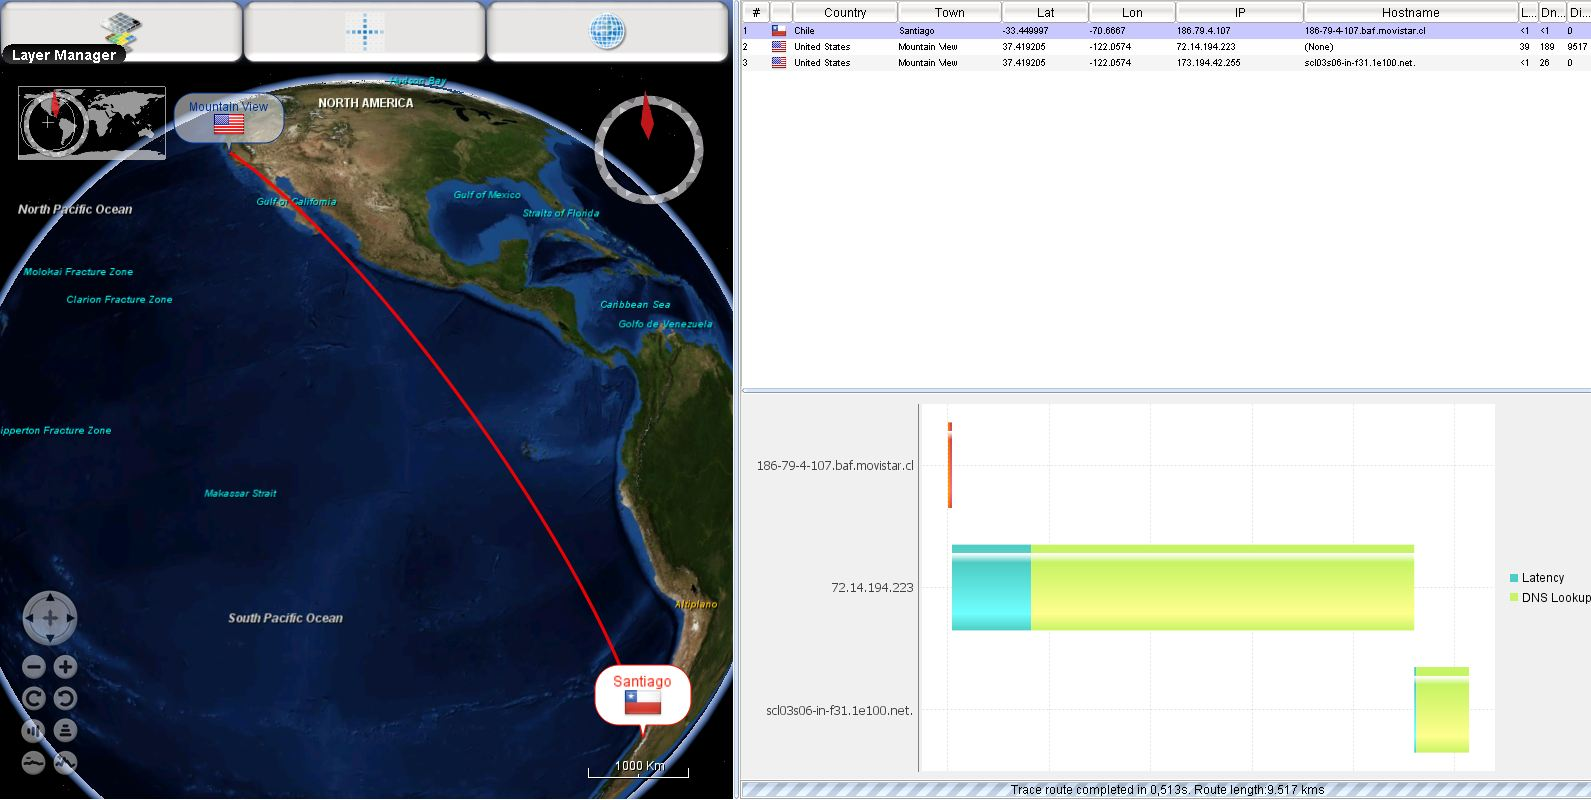
\includegraphics[width=1\textwidth]{google-cl.JPG}
\caption{\label{fig:google}Ss de Open Visual Traceroute de www.google.cl}
\end{figure}

\begin{figure}
\centering
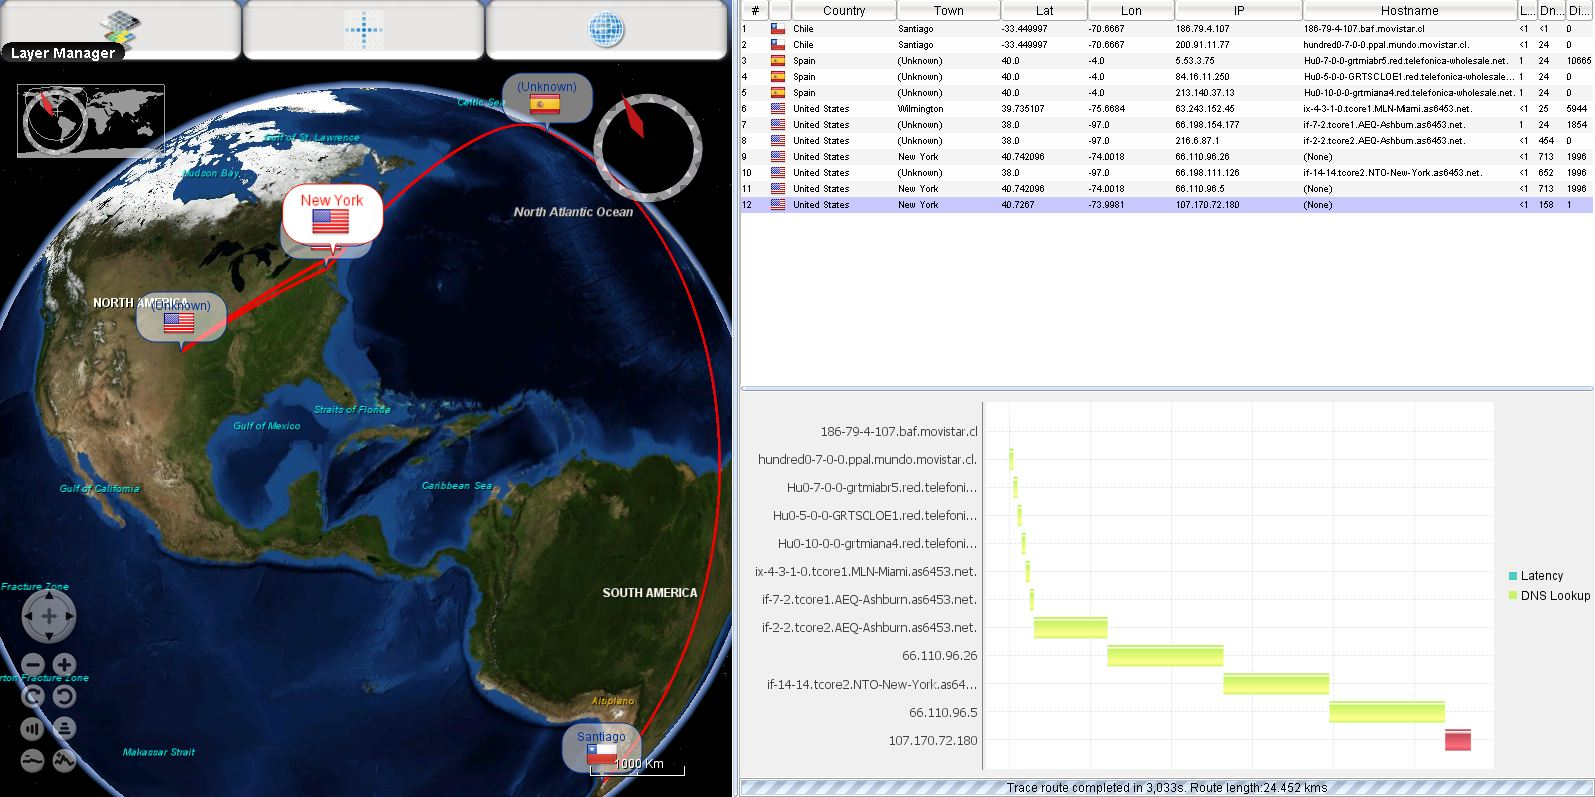
\includegraphics[width=1\textwidth]{cime.JPG}
\caption{\label{fig:cime}Ss de Open Visual Traceroute de www.cime.cl}
\end{figure}

\begin{figure}
\centering
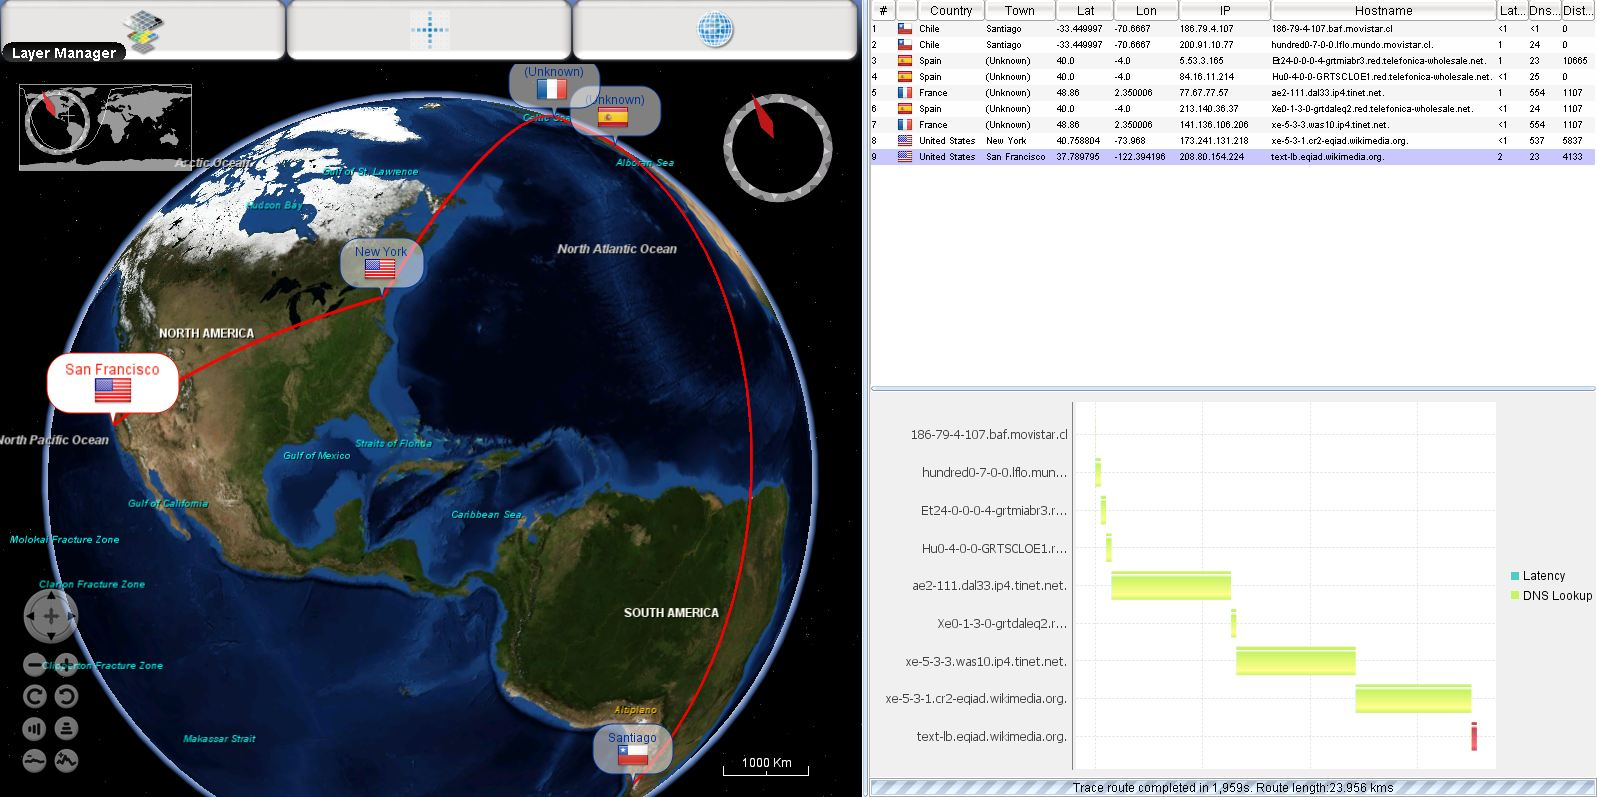
\includegraphics[width=1\textwidth]{wikipedia.JPG}
\caption{\label{fig:wiki}Ss de Open Visual Traceroute de www.wikipedia.com}
\end{figure}

\begin{figure}
\centering
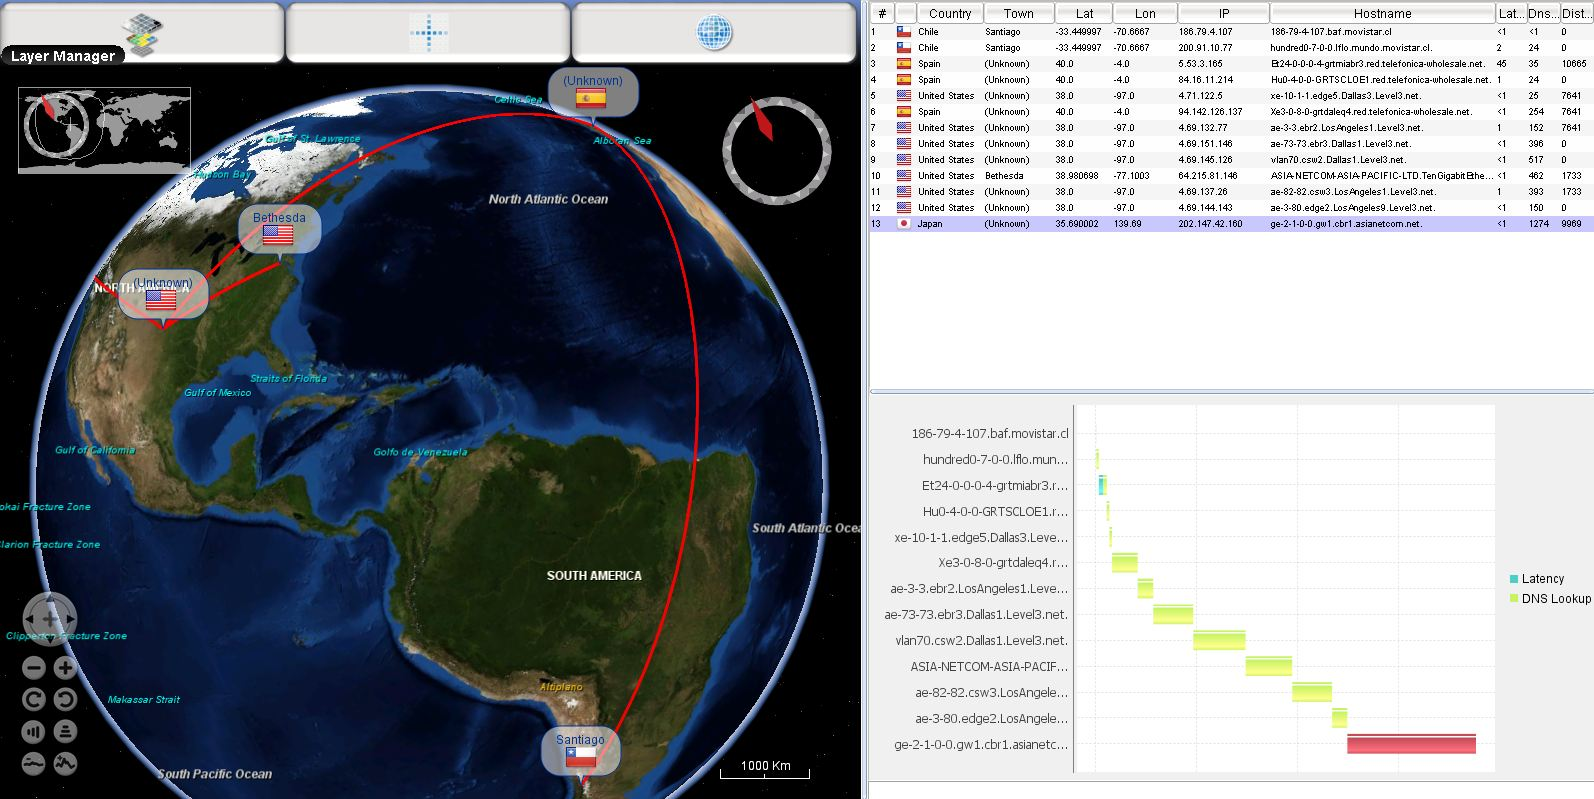
\includegraphics[width=1\textwidth]{chileembassy1.JPG}
\caption{\label{fig:embassy}Ss de Open Visual Traceroute de www.chile.embassy.gov.au}
\end{figure}

\begin{figure}
\centering
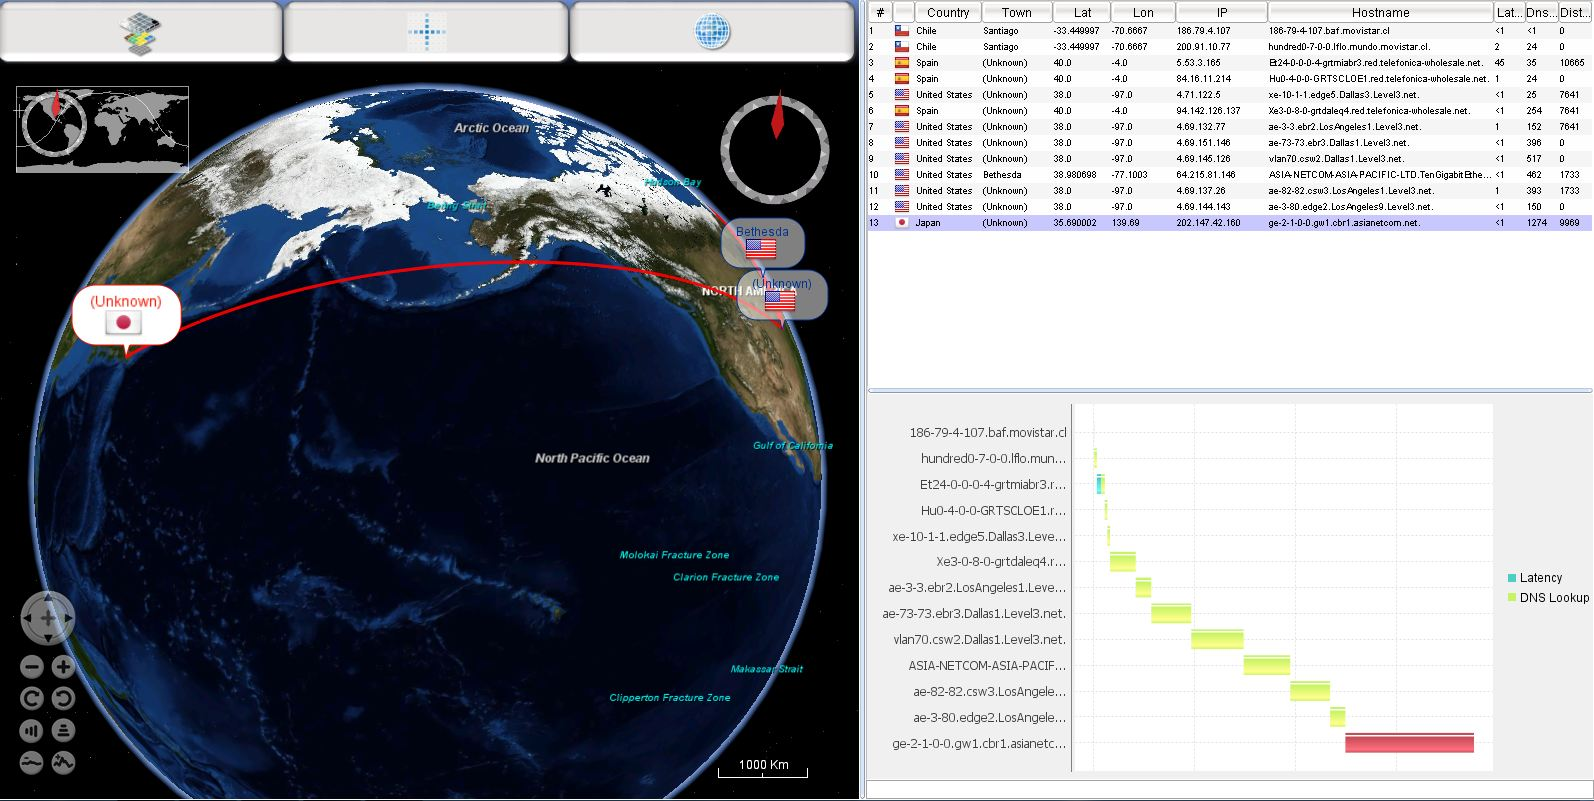
\includegraphics[width=1\textwidth]{chileembassy2.JPG}
\caption{\label{fig:embassy2}Ss de Open Visual Traceroute de www.chile.embassy.gov.au}
\end{figure}


\end{document}









































